\documentclass[aspectratio=169]{beamer}

\newif\ifshortdeck
\ifdefined\NDNSFSHORTDECK
  \shortdecktrue
\else
  \shortdeckfalse
\fi

\usetheme{default}
\usecolortheme{default}
\usefonttheme{professionalfonts}

\usepackage[T1]{fontenc}
\usepackage{lmodern}
\usepackage{tikz}
\usepackage{booktabs}
\usepackage{array}
\usepackage{tabularx}
\usepackage{graphicx}
\usetikzlibrary{positioning,arrows.meta,calc}

\graphicspath{{assets/}{../../Named_Data_Network_Service_Framework/figures/}{../../Named_Data_Network_Service_Framework/sections/}}

\definecolor{MemphisBlue}{RGB}{26,62,122}
\definecolor{LightBand}{RGB}{244,247,252}
\definecolor{SoftGray}{RGB}{90,96,108}
\definecolor{AccentGreen}{RGB}{61,130,89}
\definecolor{AccentOrange}{RGB}{194,111,46}

\setbeamertemplate{navigation symbols}{}
\setbeamertemplate{itemize item}{\color{MemphisBlue}$\blacktriangleright$}
\setbeamertemplate{itemize subitem}{\color{MemphisBlue}$\circ$}
\setbeamercolor{title}{fg=MemphisBlue}
\setbeamercolor{frametitle}{fg=MemphisBlue,bg=white}
\setbeamerfont{frametitle}{size=\Large,series=\bfseries}
\setbeamerfont{title}{size=\LARGE,series=\bfseries}
\setbeamerfont{subtitle}{size=\large}
\setbeamerfont{normal text}{size=\normalsize}
\setbeamertemplate{footline}{%
  \leavevmode%
  \hbox{%
    \begin{beamercolorbox}[wd=.78\paperwidth,ht=2.6ex,dp=1.2ex,leftskip=1.2em]{author in head/foot}%
      \scriptsize Tianxing Ma \quad PhD Proposal Defense \quad University of Memphis \quad June 2026
    \end{beamercolorbox}%
    \begin{beamercolorbox}[wd=.22\paperwidth,ht=2.6ex,dp=1.2ex,rightskip=1.2em plus1fil]{date in head/foot}%
      \scriptsize \insertframenumber/\inserttotalframenumber
    \end{beamercolorbox}%
  }%
}

\newcommand{\bluebox}[1]{%
  \begin{beamercolorbox}[rounded=true,shadow=false,sep=0.65em,wd=\linewidth]{block body}
  #1
  \end{beamercolorbox}
}
\newcommand{\slideref}[1]{\textcolor{MemphisBlue}{[#1]}}
\newcommand{\refentry}[2]{%
  \par\noindent\hangindent=0.73cm\hangafter=1%
  \makebox[0.55cm][r]{\textcolor{MemphisBlue}{[#1]}}\hspace{0.18cm}#2%
  \par\vspace{0.12cm}%
}
\setbeamercolor{block body}{bg=LightBand,fg=black}
\title{NDNSF: A Data-Centric Service Framework for Secure, Collaborative, and Dynamic Networked Applications}
\author{Tianxing Ma}
\institute{Department of Computer Science\\University of Memphis\\[0.4em]Advisor: Dr. Lan Wang}
\date{PhD Proposal Defense\\June 2026}

\begin{document}

\begin{frame}[plain]
  \titlepage
\end{frame}

\ifshortdeck
\begin{frame}{Proposal Defense Roadmap}
\begin{enumerate}
  \item \textbf{Motivation and gap}
  \item \textbf{NDNSF foundation and completed v0.1 evidence}
  \item \textbf{Post-v0.1 collaboration plan and proposed enforcement}
  \item \textbf{UAV and distributed-inference validation}
  \item \textbf{Evaluation, risks, and Spring 2027 timeline}
\end{enumerate}
\vspace{0.45cm}
\bluebox{NDNSF is the dissertation contribution; UAV and DI expose requirements and provide evidence.}
\end{frame}

\begin{frame}{Service Framework Problem}
\small
\begin{columns}[T,onlytextwidth]
\column{0.48\linewidth}
\bluebox{\textbf{What a service framework must provide}}
\begin{itemize}
  \item Discover, authorize, invoke, and compose services
  \item Observe readiness and select Providers
  \item Manage retries, security, and data transfer
\end{itemize}

\column{0.49\linewidth}
\bluebox{\textbf{Friction in endpoint-oriented designs}}
\begin{itemize}
  \item Calls bind to hosts, processes, brokers, or channels
  \item Discovery, identity, and trust sit outside invocation
  \item Stored or cached objects need separate protection
\end{itemize}
\end{columns}
\vspace{0.28cm}
\bluebox{Dynamic multi-Provider applications still bridge endpoints, service policy, trust, and data by hand.}
\end{frame}
\else
\begin{frame}{What is a service framework?}
\textbf{A service framework is a set of application-layer protocols and
libraries that turns distributed functions into reusable services.}

\vspace{0.65em}
\begin{itemize}
  \item It defines how applications discover, authorize, invoke, and compose services.
  \item It hides provider location and implementation details behind service interfaces and policies.
  \item It manages application concerns such as provider readiness, selection, retries, security, and data transfer.
  \item It is useful in UAV control, edge AI inference, storage, sensing, robotics, and many other applications.
\end{itemize}
\end{frame}

\begin{frame}{Issues with IP-Based Service Frameworks}
\small
\begin{itemize}
  \item \textbf{Endpoint-oriented invocation:} service calls commonly resolve to reachable hosts, processes, brokers, or endpoint abstractions.
  \item \textbf{Channel/session-centered security:} TLS protects communication channels; stored or cached objects need separate object-level protection.
  \item \textbf{Service semantics outside invocation:} identity, trust, network reachability, and service discovery are configured outside the service invocation.
  \item \textbf{Fundamental issue:} mismatch between IP's host-centric model and service-oriented applications' data-centric needs.
\end{itemize}

\vspace{0.35cm}
\bluebox{Existing tools solve pieces of the problem; applications still bridge hosts, services, trust, and data by hand.}
\end{frame}

\begin{frame}{Proposal Defense Roadmap}
\begin{enumerate}
  \item \textbf{Named Data Networking (NDN)} \slideref{1}: background and motivation.
  \item \textbf{Research gap:} what service-layer semantics are missing.
  \item \textbf{Framework:} NDN Service Framework (NDNSF) core design and completed foundation.
  \item \textbf{Workloads:} UAV network application and distributed inference as validation cases.
  \item \textbf{Plan:} evaluation matrix, remaining work, risks, and timeline.
\end{enumerate}
\vspace{0.55cm}
\bluebox{The central claim is that NDNSF is the dissertation contribution; the applications validate and refine the framework.}
\end{frame}
\fi

\ifshortdeck
\begin{frame}{Why NDN for Services}
\vspace{-0.15cm}
\begin{columns}[T,onlytextwidth]
\column{0.47\linewidth}
\begin{center}
\resizebox{0.98\linewidth}{!}{%
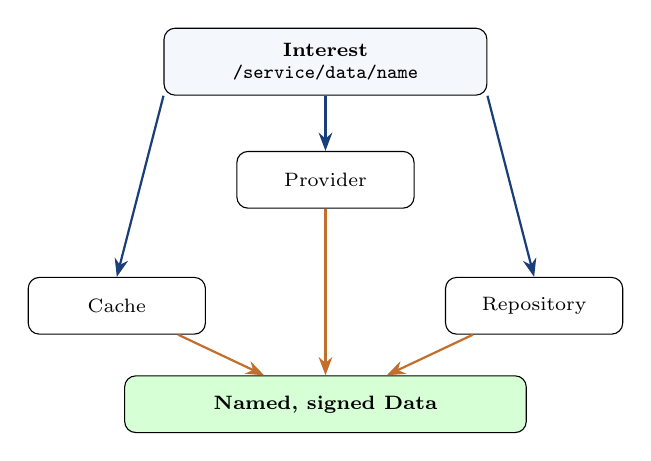
\begin{tikzpicture}[font=\scriptsize, every node/.style={align=center}]
  \node[draw, rounded corners, fill=LightBand, minimum width=4.1cm,
        minimum height=0.85cm] (interest) at (0,1.35)
        {\textbf{Interest}\\\texttt{/service/data/name}};
  \node[draw, rounded corners, fill=white, minimum width=2.25cm,
        minimum height=0.72cm] (provider) at (0,-0.15) {Provider};
  \node[draw, rounded corners, fill=white, minimum width=2.25cm,
        minimum height=0.72cm] (cache) at (-2.65,-1.75) {Cache};
  \node[draw, rounded corners, fill=white, minimum width=2.25cm,
        minimum height=0.72cm] (repo) at (2.65,-1.75) {Repository};
  \draw[-{Stealth}, thick, MemphisBlue] (interest) -- (provider);
  \draw[-{Stealth}, thick, MemphisBlue] (interest.south west) -- (cache.north);
  \draw[-{Stealth}, thick, MemphisBlue] (interest.south east) -- (repo.north);
  \node[draw, rounded corners, fill=green!16, minimum width=5.1cm,
        minimum height=0.72cm] (data) at (0,-3.0)
        {\textbf{Named, signed Data}};
  \draw[-{Stealth}, thick, AccentOrange] (provider) -- (data);
  \draw[-{Stealth}, thick, AccentOrange] (cache) -- (data);
  \draw[-{Stealth}, thick, AccentOrange] (repo) -- (data);
\end{tikzpicture}
}
\end{center}

\column{0.50\linewidth}
\small
\begin{itemize}
  \item NDN \slideref{1} lets consumers request \textbf{named Data}, not a host session.
  \item Data signatures remain verifiable across paths and storage.
  \item A Provider, cache, or repository can satisfy a matching Interest.
  \item Name-based retrieval reduces dependence on a fixed endpoint.
\end{itemize}
\end{columns}

\vspace{0.08cm}
\bluebox{\scriptsize NDN supplies named retrieval and object authenticity; NDNSF defines the service and collaboration semantics above those primitives.}
\end{frame}

\begin{frame}{NDN Packets and Service Data}
\vspace{-0.12cm}
\begin{columns}[T,onlytextwidth]
\column{0.46\linewidth}
\small
\begin{tabularx}{\linewidth}{>{\bfseries}p{0.21\linewidth}X}
\toprule
Interest & Name of desired Data plus optional selectors and parameters.\\
\midrule
Data & Name, content, metadata, and producer signature.\\
\bottomrule
\end{tabularx}

\vspace{0.35cm}
\begin{center}
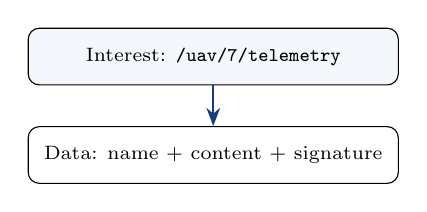
\begin{tikzpicture}[font=\scriptsize, every node/.style={align=center}]
  \node[draw, rounded corners, fill=LightBand, minimum width=4.7cm,
        minimum height=0.72cm] (i) at (0,0.8) {Interest: \texttt{/uav/7/telemetry}};
  \node[draw, rounded corners, fill=white, minimum width=4.7cm,
        minimum height=0.72cm] (d) at (0,-0.45) {Data: name + content + signature};
  \draw[-{Stealth}, thick, MemphisBlue] (i) -- (d);
\end{tikzpicture}
\end{center}

\column{0.51\linewidth}
\small
\textbf{Examples of service-relevant Named Data}
\begin{itemize}
  \item \texttt{/uav/7/telemetry/v=1042}
  \item \texttt{/uav/7/video/frame=918/seg=3}
  \item NDNSF Request, ACK, Selection, and Response
  \item model, tensor, and result artifacts
\end{itemize}
\end{columns}

\vspace{0.18cm}
\bluebox{\scriptsize NDN \slideref{1} represents business inputs, service messages, and intermediate results as independently verifiable Named Data.}
\end{frame}

\begin{frame}{Supporting NDN Primitives}
\vspace{0.10cm}
\begin{columns}[T,onlytextwidth]
\column{0.31\linewidth}
\begin{block}{NDN Sync \slideref{2} / SVS \slideref{3}}
\small Participants announce name and sequence-state changes so peers can fetch missing Data.
\end{block}

\column{0.31\linewidth}
\begin{block}{Data signatures \slideref{1}}
\small Consumers verify producer identity and object integrity whether Data is direct or cached.
\end{block}

\column{0.31\linewidth}
\begin{block}{NAC \slideref{4} / \mbox{NAC-ABE \slideref{5,19}}}
\small Name-based encryption policy determines which identities can decrypt protected Data.
\end{block}
\end{columns}

\vspace{0.32cm}
\bluebox{\scriptsize These primitives disseminate and protect individual objects; by themselves they do not assign Provider roles or authorize dependency edges in a multi-Provider execution.}
\end{frame}
\else
\begin{frame}{Why NDN Helps}
\textbf{NDN \slideref{1} changes the narrow waist from host-addressed packets to named,
secured data chunks.}

\vspace{0.10cm}
\begin{columns}[T,onlytextwidth]
\column{0.43\linewidth}
\begin{center}
\resizebox{0.97\linewidth}{!}{%
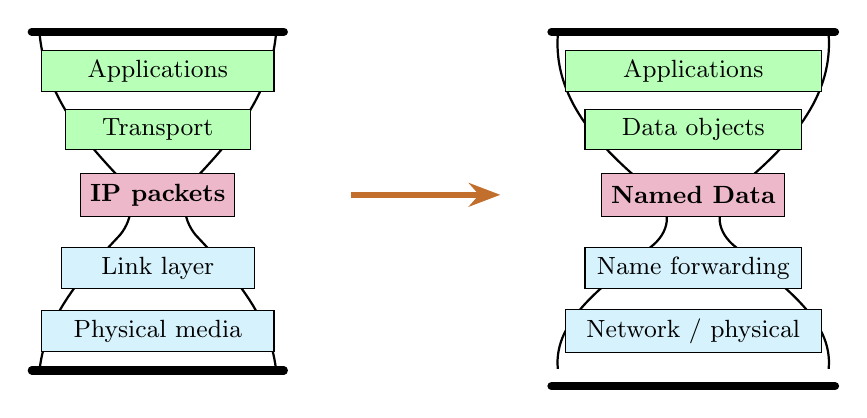
\begin{tikzpicture}[font=\small, every node/.style={align=center}]
\tikzset{
  top/.style={draw, fill=green!28, minimum height=0.34cm},
  waist/.style={draw, fill=purple!28, minimum height=0.55cm, font=\bfseries\small},
  bottom/.style={draw, fill=cyan!16, minimum height=0.34cm},
  hourcap/.style={line width=3pt, line cap=round},
  arrow/.style={-{Stealth[length=4mm,width=3mm]}, line width=2.2pt, AccentOrange}
}
  \def\lx{-3.4}
  \def\rx{3.4}

  % IP hourglass
  \draw[thick] (\lx-1.50,2.28)
    .. controls (\lx-1.42,1.50) and (\lx-0.95,0.96) .. (\lx-0.48,0.46)
    .. controls (\lx-0.30,0.24) and (\lx-0.30,-0.04) .. (\lx-0.48,-0.26)
    .. controls (\lx-0.95,-0.76) and (\lx-1.42,-1.28) .. (\lx-1.50,-1.96);
  \draw[thick] (\lx+1.50,2.28)
    .. controls (\lx+1.42,1.50) and (\lx+0.95,0.96) .. (\lx+0.48,0.46)
    .. controls (\lx+0.30,0.24) and (\lx+0.30,-0.04) .. (\lx+0.48,-0.26)
    .. controls (\lx+0.95,-0.76) and (\lx+1.42,-1.28) .. (\lx+1.50,-1.96);
  \node[top, minimum width=2.95cm] at (\lx,1.82) {Applications};
  \node[top, minimum width=2.35cm] at (\lx,1.08) {Transport};
  \node[waist, minimum width=1.32cm] at (\lx,0.25) {IP packets};
  \node[bottom, minimum width=2.45cm] at (\lx,-0.68) {Link layer};
  \node[bottom, minimum width=2.95cm] at (\lx,-1.48) {Physical media};
  \draw[hourcap] (\lx-1.6,2.32) -- (\lx+1.6,2.32);
  \draw[hourcap] (\lx-1.6,-1.98) -- (\lx+1.6,-1.98);

  % NDN hourglass
  \draw[thick] (\rx-1.72,2.28)
    .. controls (\rx-1.78,1.40) and (\rx-1.10,0.78) .. (\rx-0.50,0.28)
    .. controls (\rx-0.28,0.08) and (\rx-0.28,-0.18) .. (\rx-0.50,-0.38)
    .. controls (\rx-1.10,-0.88) and (\rx-1.78,-1.32) .. (\rx-1.72,-1.96);
  \draw[thick] (\rx+1.72,2.28)
    .. controls (\rx+1.78,1.40) and (\rx+1.10,0.78) .. (\rx+0.50,0.28)
    .. controls (\rx+0.28,0.08) and (\rx+0.28,-0.18) .. (\rx+0.50,-0.38)
    .. controls (\rx+1.10,-0.88) and (\rx+1.78,-1.32) .. (\rx+1.72,-1.96);
  \node[top, minimum width=3.25cm] at (\rx,1.82) {Applications};
  \node[top, minimum width=2.75cm] at (\rx,1.08) {Data objects};
  \node[waist, minimum width=1.72cm] at (\rx,0.25) {Named Data};
  \node[bottom, minimum width=2.75cm] at (\rx,-0.68) {Name forwarding};
  \node[bottom, minimum width=3.25cm] at (\rx,-1.48) {Network / physical};
  \draw[hourcap] (\rx-1.8,2.32) -- (\rx+1.8,2.32);
  \draw[hourcap] (\rx-1.8,-2.18) -- (\rx+1.8,-2.18);

  \draw[arrow] (-0.95,0.25) -- (0.95,0.25);
\end{tikzpicture}%
}
\end{center}

\column{0.54\linewidth}
\scriptsize
\begin{tabularx}{\linewidth}{>{\raggedright\arraybackslash}p{0.43\linewidth}>{\raggedright\arraybackslash}X}
\toprule
\textbf{IP-centered issue} & \textbf{NDN mechanism}\\
\midrule
Calls resolve to hosts or endpoints &
Interests retrieve named Data from any valid producer or cache.\\
\addlinespace[0.25em]
Security protects a channel &
Every Data packet carries a verifiable signature.\\
\addlinespace[0.25em]
Failover and mobility need endpoint repair &
Name-based forwarding can use another path or producer.\\
\addlinespace[0.25em]
Objects need separate storage/distribution logic &
Named Data can be cached, stored, and fetched unchanged.\\
\bottomrule
\end{tabularx}
\end{columns}

\vspace{0cm}
\bluebox{\scriptsize NDN supplies named retrieval and data-centric security; NDNSF adds the missing service semantics: authorization, readiness, invocation, and provider coordination.}
\end{frame}

\begin{frame}{NDN Packet Model}
\vspace{-0.2cm}
\begin{columns}[T,onlytextwidth]
\column{0.48\linewidth}
\begin{center}
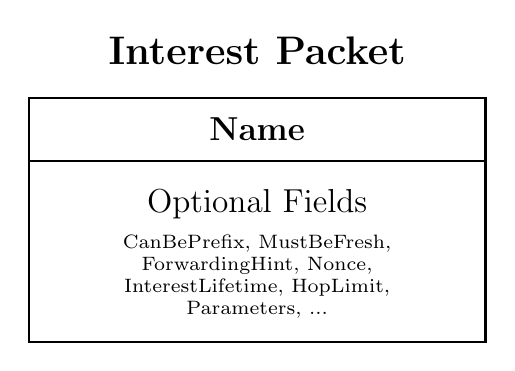
\begin{tikzpicture}[x=1cm,y=1cm, every node/.style={align=center}]
  \node[font=\Large\bfseries] at (0,2.05) {Interest Packet};
  \draw[thick] (-2.9,1.45) rectangle (2.9,-1.65);
  \draw[thick] (-2.9,0.65) -- (2.9,0.65);
  \node[font=\large\bfseries] at (0,1.05) {Name};
  \node[font=\large] at (0,0.10) {Optional Fields};
  \node[font=\scriptsize] at (0,-0.82) {CanBePrefix, MustBeFresh,\\ForwardingHint, Nonce,\\InterestLifetime, HopLimit,\\Parameters, ...};
\end{tikzpicture}
\end{center}

\column{0.48\linewidth}
\begin{center}
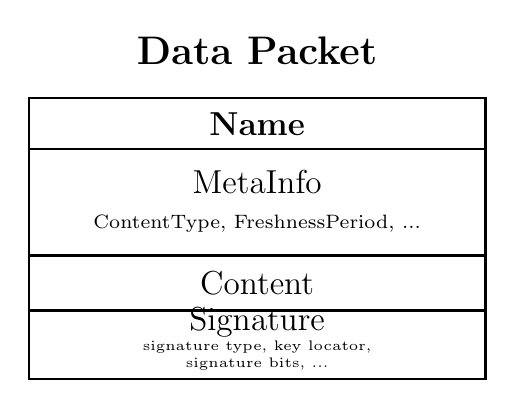
\begin{tikzpicture}[x=1cm,y=1cm, every node/.style={align=center}]
  \node[font=\Large\bfseries] at (0,2.05) {Data Packet};
  \draw[thick] (-2.9,1.45) rectangle (2.9,-2.12);
  \draw[thick] (-2.9,0.80) -- (2.9,0.80);
  \draw[thick] (-2.9,-0.55) -- (2.9,-0.55);
  \draw[thick] (-2.9,-1.25) -- (2.9,-1.25);
  \node[font=\large\bfseries] at (0,1.12) {Name};
  \node[font=\large] at (0,0.38) {MetaInfo};
  \node[font=\scriptsize] at (0,-0.15) {ContentType, FreshnessPeriod, ...};
  \node[font=\large] at (0,-0.90) {Content};
  \node[font=\large] at (0,-1.40) {Signature};
  \node[font=\tiny] at (0,-1.82) {signature type, key locator,\\signature bits, ...};
\end{tikzpicture}
\end{center}
\end{columns}

\vspace{0.12cm}
\bluebox{In NDN \slideref{1}, Interests name desired Data; Data packets carry names, content, metadata, and signatures.}
\end{frame}

\begin{frame}{NDN Packet Example: UAV Telemetry and Video}
\vspace{-0.1cm}
\begin{columns}[T,onlytextwidth]
\column{0.49\linewidth}
\begin{center}
\textbf{Telemetry status}\\[0.25em]
\resizebox{0.96\linewidth}{!}{%
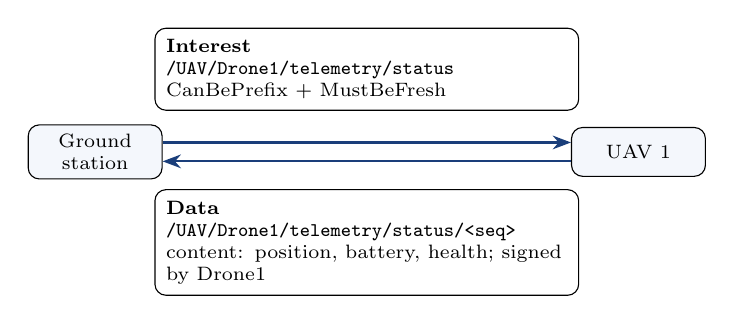
\begin{tikzpicture}[font=\scriptsize, every node/.style={align=center}]
\tikzset{
  nodebox/.style={draw, rounded corners, fill=LightBand, minimum width=1.7cm, minimum height=0.62cm},
  labelbox/.style={draw, rounded corners, fill=white, text width=5.1cm, align=left, inner sep=4pt},
  arr/.style={-{Stealth}, thick, MemphisBlue}
}
  \node[nodebox] (gs) at (0,0) {Ground\\station};
  \node[nodebox] (uav) at (6.9,0) {UAV 1};
  \node[labelbox] (interest) at (3.45,1.05) {\textbf{Interest}\\\texttt{/UAV/Drone1/telemetry/status}\\CanBePrefix + MustBeFresh};
  \node[labelbox] (data) at (3.45,-1.15) {\textbf{Data}\\\texttt{/UAV/Drone1/telemetry/status/<seq>}\\content: position, battery, health; signed by Drone1};
  \draw[arr] ($(gs.east)+(0,0.12)$) -- ($(uav.west)+(0,0.12)$);
  \draw[arr] ($(uav.west)+(0,-0.12)$) -- ($(gs.east)+(0,-0.12)$);
\end{tikzpicture}%
}
\end{center}

\column{0.49\linewidth}
\begin{center}
\textbf{Video segment}\\[0.25em]
\resizebox{0.96\linewidth}{!}{%
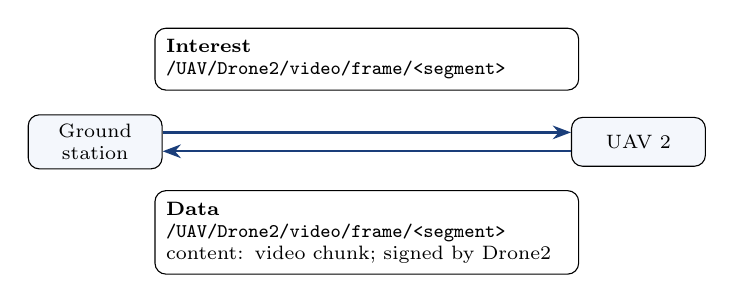
\begin{tikzpicture}[font=\scriptsize, every node/.style={align=center}]
\tikzset{
  nodebox/.style={draw, rounded corners, fill=LightBand, minimum width=1.7cm, minimum height=0.62cm},
  labelbox/.style={draw, rounded corners, fill=white, text width=5.1cm, align=left, inner sep=4pt},
  arr/.style={-{Stealth}, thick, MemphisBlue}
}
  \node[nodebox] (gs) at (0,0) {Ground\\station};
  \node[nodebox] (uav) at (6.9,0) {UAV 2};
  \node[labelbox] (interest) at (3.45,1.05) {\textbf{Interest}\\\texttt{/UAV/Drone2/video/frame/<segment>}};
  \node[labelbox] (data) at (3.45,-1.15) {\textbf{Data}\\\texttt{/UAV/Drone2/video/frame/<segment>}\\content: video chunk; signed by Drone2};
  \draw[arr] ($(gs.east)+(0,0.12)$) -- ($(uav.west)+(0,0.12)$);
  \draw[arr] ($(uav.west)+(0,-0.12)$) -- ($(gs.east)+(0,-0.12)$);
\end{tikzpicture}%
}
\end{center}
\end{columns}

\vspace{0.15cm}
\small
\textbf{Takeaway:} applications name desired data; any valid producer, cache, or repository can return signed Data with a matching name.
\end{frame}

\begin{frame}{NDN Data-Centric Security}
\textbf{In NDN \slideref{1}, security is attached to Data, not to the channel that carried it.}

\vspace{0.35cm}
\begin{center}
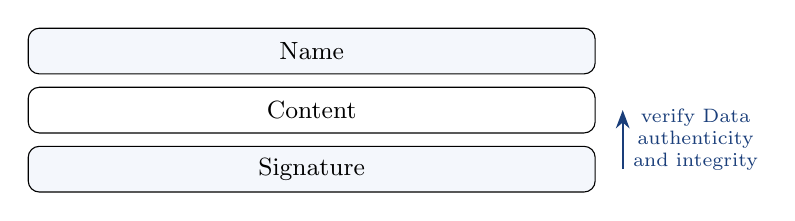
\begin{tikzpicture}[font=\small, every node/.style={align=center}]
  \node[draw, rounded corners, fill=LightBand, minimum width=7.2cm, minimum height=0.58cm] (n) at (0,1.0) {Name};
  \node[draw, rounded corners, fill=white, minimum width=7.2cm, minimum height=0.58cm] (c) at (0,0.25) {Content};
  \node[draw, rounded corners, fill=LightBand, minimum width=7.2cm, minimum height=0.58cm] (s) at (0,-0.50) {Signature};
  \draw[-{Stealth}, thick, MemphisBlue] (3.95,-0.50) -- node[right, font=\scriptsize]{verify Data\\authenticity\\and integrity} (3.95,0.25);
\end{tikzpicture}
\end{center}

\vspace{0.35cm}
\begin{itemize}
  \item A consumer can verify Data after retrieval.
  \item Verification still works through caches, repositories, and alternate paths.
  \item Access-control policy is a higher-layer question, to be explained later with NDNSF.
\end{itemize}
\end{frame}

\begin{frame}{NDN Sync and State Vector Sync}
\textbf{NDN Sync \slideref{2} communicates dataset changes; State Vector Sync
(SVS) \slideref{3} synchronizes Alice, Bob, and Ted's knowledge of that dataset.}

\vspace{0.03cm}
\begin{center}
\resizebox{0.90\linewidth}{!}{%
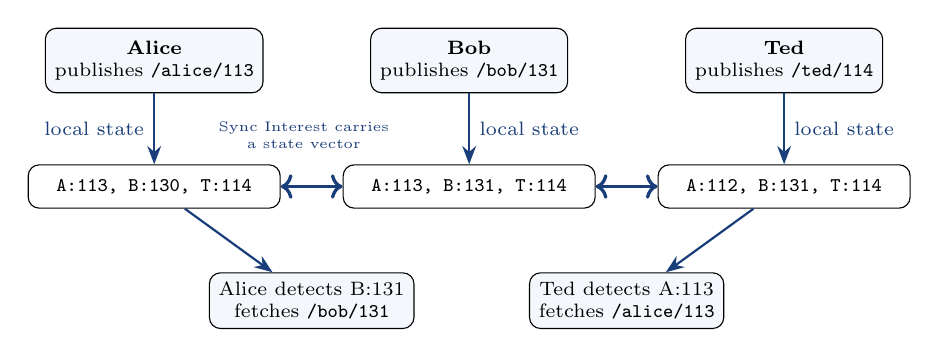
\begin{tikzpicture}[font=\scriptsize, every node/.style={align=center}]
\tikzset{
  peer/.style={draw, rounded corners, fill=LightBand, minimum width=2.45cm, minimum height=0.82cm},
  vector/.style={draw, rounded corners, fill=white, minimum width=3.2cm, minimum height=0.55cm},
  data/.style={draw, rounded corners, fill=LightBand, minimum width=2.25cm, minimum height=0.55cm},
  arr/.style={-{Stealth}, thick, MemphisBlue}
}
  \node[peer] (alice) at (-4.0,1.55) {\textbf{Alice}\\publishes \texttt{/alice/113}};
  \node[peer] (bob) at (0,1.55) {\textbf{Bob}\\publishes \texttt{/bob/131}};
  \node[peer] (ted) at (4.0,1.55) {\textbf{Ted}\\publishes \texttt{/ted/114}};

  \node[vector] (av) at (-4.0,-0.05) {\texttt{A:113, B:130, T:114}};
  \node[vector] (bv) at (0,-0.05) {\texttt{A:113, B:131, T:114}};
  \node[vector] (tv) at (4.0,-0.05) {\texttt{A:112, B:131, T:114}};
  \draw[arr] (alice) -- node[left]{local state} (av);
  \draw[arr] (bob) -- node[right]{local state} (bv);
  \draw[arr] (ted) -- node[right]{local state} (tv);

  \node[fill=white, text=MemphisBlue, font=\tiny, inner sep=1.5pt] at (-2.1,0.60)
    {Sync Interest carries\\a state vector};
  \draw[<->, very thick, MemphisBlue] (av) -- (bv);
  \draw[<->, very thick, MemphisBlue] (bv) -- (tv);

  \node[data] (fetchb) at (-2.0,-1.50) {Alice detects B:131\\fetches \texttt{/bob/131}};
  \node[data] (fetcha) at (2.0,-1.50) {Ted detects A:113\\fetches \texttt{/alice/113}};
  \draw[arr] (av) -- (fetchb);
  \draw[arr] (tv) -- (fetcha);
\end{tikzpicture}%
}
\end{center}

\vspace{0.03cm}
\bluebox{\scriptsize Each participant compares received and local sequence numbers, identifies missing names, and fetches the corresponding Data. All three converge on the same dataset without a central broker.}
\end{frame}

\begin{frame}{Name-Based Access Control: NAC}
\textbf{NAC \slideref{4} protects named NDN Data; NAC-ABE \slideref{5,19}
applies attribute-based decryption policy.}

\vspace{0.2cm}
\begin{columns}[T,onlytextwidth]
\column{0.44\linewidth}
\small
\begin{itemize}
  \item Content is encrypted at production, so Data stays protected in caches and repositories.
  \item NDN names express policy granularity and key names for automatic key retrieval.
  \item NAC-ABE uses attributes to decide which identities can decrypt named Data.
\end{itemize}

\column{0.53\linewidth}
\begin{center}
\resizebox{\linewidth}{!}{%
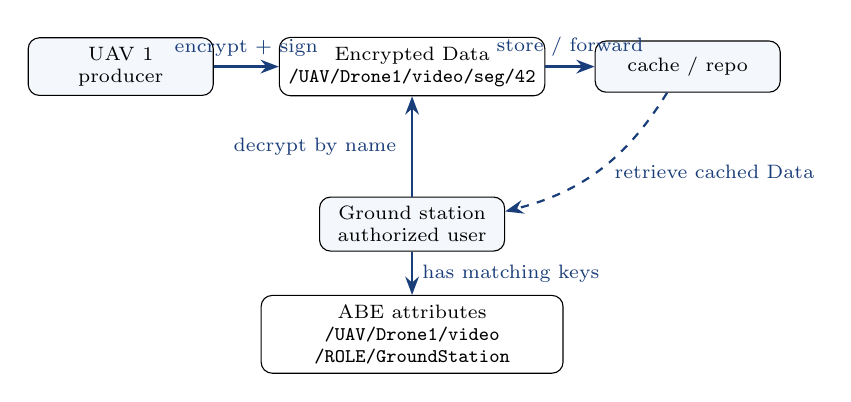
\begin{tikzpicture}[font=\scriptsize, every node/.style={align=center}]
\tikzset{
  box/.style={draw, rounded corners, fill=LightBand, minimum width=2.35cm, minimum height=0.65cm},
  whitebox/.style={draw, rounded corners, fill=white, minimum width=2.6cm, minimum height=0.65cm},
  arr/.style={-{Stealth}, thick, MemphisBlue}
}
  \node[box] (uav) at (0,1.7) {UAV 1\\producer};
  \node[whitebox] (data) at (3.7,1.7) {Encrypted Data\\\texttt{/UAV/Drone1/video/seg/42}};
  \node[box] (repo) at (7.2,1.7) {cache / repo};
  \node[box] (gs) at (3.7,-0.3) {Ground station\\authorized user};
  \node[whitebox, text width=3.6cm] (attr) at (3.7,-1.7) {ABE attributes\\\texttt{/UAV/Drone1/video}\\\texttt{/ROLE/GroundStation}};

  \draw[arr] (uav) -- node[above]{encrypt + sign} (data);
  \draw[arr] (data) -- node[above]{store / forward} (repo);
  \draw[arr] (gs) -- node[right]{has matching keys} (attr);
  \draw[arr] (gs) -- node[left, xshift=-2pt]{decrypt by name} (data);
  \draw[arr, dashed] (repo) to[bend left=22]
    node[pos=0.52, right, xshift=3pt]{retrieve cached Data} (gs);
\end{tikzpicture}%
}
\end{center}
\end{columns}

\vspace{0.12cm}
\bluebox{\scriptsize Example: UAV telemetry or video Data can be cached anywhere, but only ground stations with matching NAC-ABE attributes can decrypt it.}
\end{frame}
\fi

\begin{frame}{Research Gap}
\begin{center}
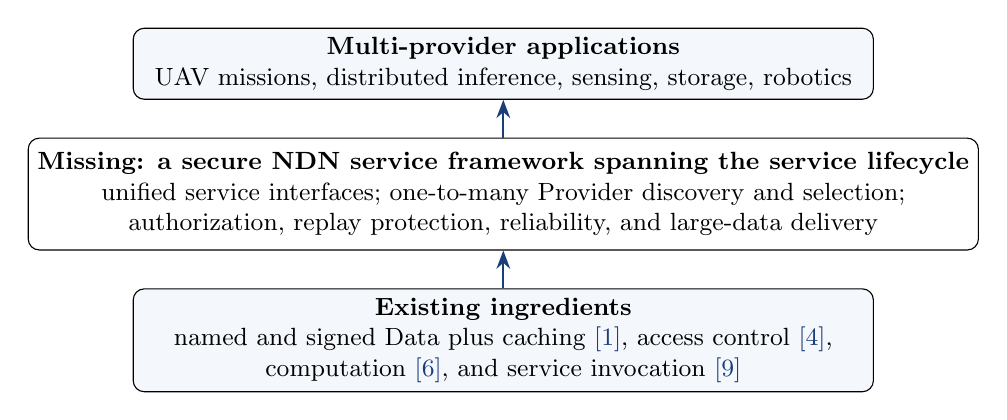
\begin{tikzpicture}[node distance=0.48cm, every node/.style={font=\small, align=center}]
  \node[draw, rounded corners, fill=LightBand, minimum width=9.4cm, minimum height=0.72cm] (app) {\textbf{Multi-provider applications}\\UAV missions, distributed inference, sensing, storage, robotics};
  \node[draw, rounded corners, fill=white, below=of app, minimum width=9.4cm, minimum height=1.42cm] (gap) {\textbf{Missing: a secure NDN service framework spanning the service lifecycle}\\unified service interfaces; one-to-many Provider discovery and selection;\\authorization, replay protection, reliability, and large-data delivery};
  \node[draw, rounded corners, fill=LightBand, below=of gap, minimum width=9.4cm, minimum height=0.82cm] (ndn) {\textbf{Existing ingredients}\\named and signed Data plus caching \slideref{1}, access control \slideref{4},\\computation \slideref{6}, and service invocation \slideref{9}};
  \draw[-{Stealth}, thick, MemphisBlue] (ndn) -- (gap);
  \draw[-{Stealth}, thick, MemphisBlue] (gap) -- (app);
\end{tikzpicture}
\end{center}
\bluebox{NDNSF v0.1 supplies the core framework functions; the proposed dissertation work extends them to multi-role collaboration and verifies Data flow between assigned roles.}
\end{frame}

\begin{frame}{Related Work: NDN Service Framework Directions}
\scriptsize
\begin{columns}[T,onlytextwidth]
\column{0.48\linewidth}
\bluebox{\textbf{Computation / composition:} NFN \slideref{6}, NFaaS \slideref{7}, CFEC \slideref{8}, CFN \slideref{14}, CaSCON \slideref{15}, and data-centric composition \slideref{21}\\Named functions, placement, computation graphs, and dependency-aware composition.}
\vspace{0.12cm}
\bluebox{\textbf{Invocation:} RICE \slideref{9}, NSC \slideref{10}\\Named remote calls and execution; do not by themselves enforce a late-bound multi-role Data-admission policy.}
\column{0.48\linewidth}
\bluebox{\textbf{Content authorization:} NAC \slideref{4}, NAC-ABE \slideref{5,19}, Trust Schema \slideref{16}, and access-controlled derived Data \slideref{20}\\Protect content and constrain valid signers; policy is not derived from a runtime collaboration plan.}
\vspace{0.12cm}
\bluebox{\textbf{Application-specific:} MIA-NDN \slideref{11}, DNMP \slideref{12}, SECaaS \slideref{13}\\Targets aggregation, measurement, or edge security.}
\end{columns}
\vspace{0.12cm}
\bluebox{\scriptsize\raggedright
\textbf{Targeted collaboration gap.} NDNSF v0.1 already covers secure invocation, runtime Provider discovery and selection, authorization, replay protection, and reliable Data delivery.\\
The proposed extension addresses a narrower missing function: after runtime ACKs, derive a multi-role dependency plan and admit intermediate Data only when its name, signer, assigned role, dependency edge, and request context match, including Data retrieved from an NDN cache.}
\end{frame}

\begin{frame}{NDNSF Contribution}
\scriptsize
\renewcommand{\arraystretch}{1.02}
\begin{tabularx}{\linewidth}{>{\raggedright\arraybackslash}p{0.28\linewidth}>{\raggedright\arraybackslash}X}
\toprule
\textbf{Framework function} & \textbf{NDNSF contribution}\\
\midrule
\textbf{Service interfaces and invocation}\\v0.1 &
Generic C++ and Python APIs support Request, ACK, Selection, Response, and Targeted invocation without service-specific stubs; C++ also provides trusted same-process local calls.\\
\midrule
\textbf{One-to-many service model}\\v0.1 &
One named Request reaches willing Providers; applications use built-in or customizable Provider-selection strategies.\\
\midrule
\textbf{Security and authorization}\\v0.1 &
Name-based policy, NAC-ABE, signatures, one-time tokens, and replay checks protect invocation and Data.\\
\midrule
\textbf{Reliability and data delivery}\\implemented &
SVS retry, segmented retrieval, large-object references, streaming, and bounded FEC recovery.\\
\midrule
\textbf{Multi-role collaboration}\\proposed work &
Assign willing Providers to application roles, declare allowed Data flow, and verify Data received between assigned roles.\\
\bottomrule
\end{tabularx}
\end{frame}

\ifshortdeck
\else
\begin{frame}{Dissertation Components}
\begin{center}
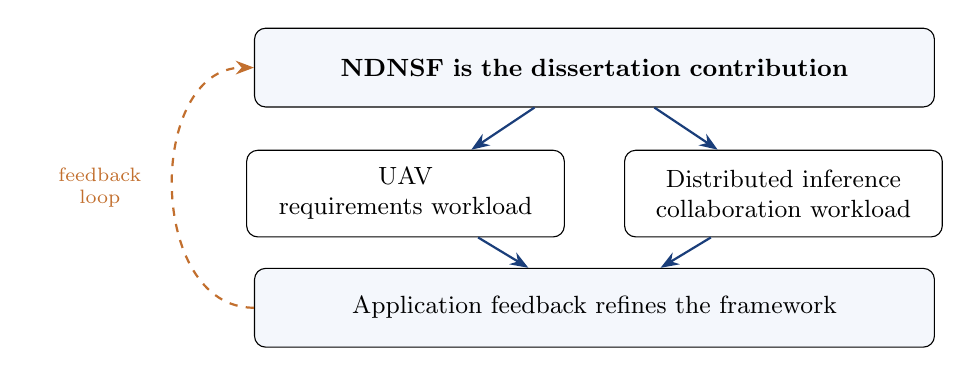
\begin{tikzpicture}[every node/.style={font=\small, align=center}]
  \node[draw, rounded corners, fill=LightBand, text width=8.4cm, minimum height=1.0cm] (core) at (0,1.6) {\textbf{NDNSF is the dissertation contribution}};
  \node[draw, rounded corners, fill=white, text width=3.8cm, minimum height=1.1cm] (uav) at (-2.4,0.0) {UAV\\requirements workload};
  \node[draw, rounded corners, fill=white, text width=3.8cm, minimum height=1.1cm] (di) at (2.4,0.0) {Distributed inference\\collaboration workload};
  \node[draw, rounded corners, fill=LightBand, text width=8.4cm, minimum height=1.0cm] (e) at (0,-1.45) {Application feedback refines the framework};
  \draw[-{Stealth}, thick, MemphisBlue] (core) -- (uav);
  \draw[-{Stealth}, thick, MemphisBlue] (core) -- (di);
  \draw[-{Stealth}, thick, MemphisBlue] (uav) -- (e);
  \draw[-{Stealth}, thick, MemphisBlue] (di) -- (e);
  \draw[-{Stealth}, thick, dashed, AccentOrange] (e.west) to[out=180,in=180,looseness=1.15]
    node[left, font=\scriptsize, text width=1.6cm]{feedback\\loop} (core.west);
\end{tikzpicture}
\end{center}
\end{frame}
\fi

\begin{frame}{Research Questions}
\small
\begin{description}
  \item[RQ1] Which service-layer functions are required to support secure invocation, dynamic multi-Provider selection, authorization, and reliable Data delivery over NDN?
  \item[RQ2] How can NDNSF assign Providers to application roles and verify that each downstream Provider accepts Data only from the Provider assigned to an authorized upstream role?
  \item[RQ3] What reliability, security, and latency tradeoffs arise from multi-Provider publication, selection, Targeted invocation, and bounded response retry or Provider reselection?
  \item[RQ4] How should mobility and control requirements in UAV network applications be supported through NDNSF?
  \item[RQ5] How should distributed inference use NDNSF to reuse model files, assign model parts to available devices at runtime, and run one model across multiple devices?
\end{description}
\vspace{0.25cm}
\bluebox{\scriptsize RQ2 tests role assignment and Data-flow verification for both directly received and cached Named Data.}
\end{frame}

\ifshortdeck
\else
\begin{frame}{Proposed Work Status and Timeline}
\scriptsize
\setlength{\tabcolsep}{3.5pt}
\renewcommand{\arraystretch}{1.10}
\begin{tabularx}{\linewidth}{>{\raggedright\arraybackslash}p{0.15\linewidth}>{\raggedright\arraybackslash}X>{\raggedright\arraybackslash}X>{\raggedright\arraybackslash}p{0.14\linewidth}}
\toprule
\textbf{Section} & \textbf{Completed Work} & \textbf{Remaining Work} & \textbf{Target}\\
\midrule
NDNSF framework &
v0.1 invocation/security; Targeted invocation; trusted local calls; large-data support; execution-plan schema &
Implement Plan-to-Data enforcement for direct and cached Data; measure security and latency overhead &
Aug. 2026\\
\midrule
UAV workload &
Control, telemetry, video, and mobility workload &
Multi-drone role/edge tests in MiniNDN \slideref{22} and PX4 SITL \slideref{23} &
Sept. 2026\\
\midrule
Distributed inference &
Planner, Repo, named dependency flow; preliminary model campaign &
Real-model and failure gates; final statistical evaluation &
Oct. 2026\\
\midrule
Evidence and chair draft &
Proposal, survey, and v0.1 manuscript &
Freeze evidence; integrate chapters; submit chair draft &
Nov.--Dec. 2026\\
\midrule
Graduation path &
Spring 2027 path and deadlines confirmed &
Committee review; February 2027 defense; corrections and ProQuest &
Jan.--Mar. 2027\\
\bottomrule
\end{tabularx}
\vspace{0.28cm}
\bluebox{\scriptsize Defense by mid-Feb. 2027; ProQuest: March 5 target, March 26 deadline; Spring 2027 graduation.}
\end{frame}
\fi

\ifshortdeck
\begin{frame}{Completed Foundation: NDNSF v0.1}
\begin{columns}[T,onlytextwidth]
\column{0.43\linewidth}
\begin{itemize}
  \item Implemented generic dynamic C++ API
  \item Multi-provider ACK collection
  \item Provider selection strategies
  \item NDN-SVS patch
  \item MiniNDN \slideref{22} evaluation
\end{itemize}

\column{0.53\linewidth}
\textbf{Provider API}\\[0.10cm]
\bluebox{\ttfamily\scriptsize
provider.addHandler\textless RequestT, ResponseT\textgreater(\\
\hspace*{0.35cm}serviceName, handler);}

\vspace{0.22cm}
\textbf{User API}\\[0.10cm]
\bluebox{\ttfamily\scriptsize
user.RequestService\textless RequestT, ResponseT\textgreater(\\
\hspace*{0.35cm}providers, serviceName, request,\\
\hspace*{0.35cm}onResponse, onTimeout, timeoutMs,\\
\hspace*{0.35cm}strategy);}
\end{columns}
\vspace{0.35cm}
\bluebox{\small NDNSF v0.1 (commit \texttt{be9421f\ldots}, tree \texttt{c9cc0c\ldots}) is the May 20 repository baseline; role-based dependency collaboration is post-v0.1 work.}
\end{frame}
\fi

\begin{frame}{NDNSF Entity Roles}
\begin{center}
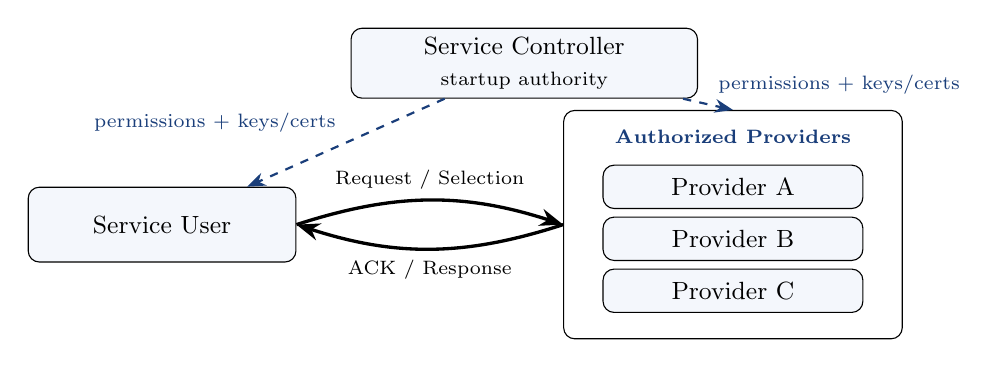
\begin{tikzpicture}[x=1cm,y=1cm, every node/.style={font=\small, align=center}]
  \node[draw, rounded corners, fill=LightBand, minimum width=4.4cm, minimum height=0.85cm] (c) at (4.6,2.05) {Service Controller\\{\scriptsize startup authority}};

  \node[draw, rounded corners, fill=LightBand, minimum width=3.4cm, minimum height=0.95cm] (u) at (0,0) {Service User};
  \node[draw, rounded corners, fill=white, minimum width=4.3cm, minimum height=2.9cm] (pg) at (7.25,0) {};
  \node[font=\scriptsize\bfseries, MemphisBlue] at (7.25,1.12) {Authorized Providers};
  \node[draw, rounded corners, fill=LightBand, minimum width=3.3cm, minimum height=0.55cm] at (7.25,0.48) {Provider A};
  \node[draw, rounded corners, fill=LightBand, minimum width=3.3cm, minimum height=0.55cm] at (7.25,-0.18) {Provider B};
  \node[draw, rounded corners, fill=LightBand, minimum width=3.3cm, minimum height=0.55cm] at (7.25,-0.84) {Provider C};

  \draw[-{Stealth}, dashed, thick, MemphisBlue] (c) -- node[above left, font=\scriptsize]{permissions + keys/certs} (u);
  \draw[-{Stealth}, dashed, thick, MemphisBlue] (c) -- node[above right, font=\scriptsize]{permissions + keys/certs} (pg.north);

  \draw[-{Stealth}, very thick] (u.east) to[bend left=18] node[above, font=\scriptsize]{Request / Selection} (pg.west);
  \draw[-{Stealth}, very thick] (pg.west) to[bend left=18] node[below, font=\scriptsize]{ACK / Response} (u.east);
\end{tikzpicture}
\end{center}
\bluebox{At startup, users and providers obtain permissions, keys, and certificates. During invocation, the user coordinates directly with providers through named Data messages.}
\end{frame}

\begin{frame}{NDNSF Invocation Workflow}
\vspace{-0.10cm}
\begin{center}
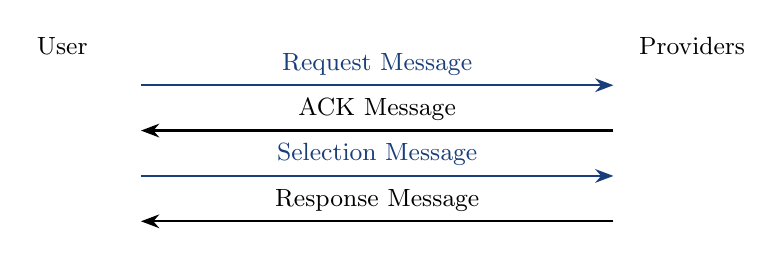
\begin{tikzpicture}[x=1cm,y=0.72cm, every node/.style={font=\small}]
  \node (u) at (0,0) {User};
  \node (p) at (8,0) {Providers};
  \draw[-{Stealth}, thick, MemphisBlue] (1,-0.7) -- node[above]{Request Message} (7,-0.7);
  \draw[-{Stealth}, thick] (7,-1.5) -- node[above]{ACK Message} (1,-1.5);
  \draw[-{Stealth}, thick, MemphisBlue] (1,-2.3) -- node[above]{Selection Message} (7,-2.3);
  \draw[-{Stealth}, thick] (7,-3.1) -- node[above]{Response Message} (1,-3.1);
\end{tikzpicture}
\end{center}

\vspace{-0.12cm}
\begin{columns}[T,onlytextwidth]
\column{0.49\linewidth}
\bluebox{\scriptsize
\textbf{Underlying NDN Sync \slideref{2}: announce, then fetch}
\begin{enumerate}
  \item Sender publishes each logical message as signed, named Data.
  \item Sync announces the new Data name.
  \item Receiver sends an Interest for that name and obtains the Data.
\end{enumerate}
}

\column{0.49\linewidth}
\bluebox{\scriptsize
\textbf{SVS \slideref{3} Pub/Sub API: combines the two-step delivery}
\begin{itemize}
  \item \texttt{publish(name, payload)} stores the Data and announces its name.
  \item \texttt{subscribe(prefix, callback)} learns the name, fetches the Data, then invokes the callback.
\end{itemize}
\textbf{The NDNSF application does not manage the fetch itself.}
}
\end{columns}

\end{frame}

\ifshortdeck
\begin{frame}{ABE-Backed Authorization: Rationale and Limits}
\vspace{-0.10cm}
\begin{columns}[T,onlytextwidth]
\column{0.48\linewidth}
\small
\textbf{Why this design?}
\begin{itemize}
  \item NAC-ABE \slideref{19} protects discovery content for authorized Providers before selection.
  \item A DKEY aggregates service permissions; identity-signing credentials are reused.
  \item Runtime status checks and key rotation support revocation, with propagation and rekeying costs.
\end{itemize}

\column{0.49\linewidth}
\scriptsize
\begin{tabularx}{\linewidth}{>{\bfseries}p{0.25\linewidth}X}
\toprule
Message & Invocation binding\\
\midrule
Request & fresh \texttt{UserToken}\\
ACK & echoed \texttt{UserToken} + fresh \texttt{ProviderToken}\\
Selection & selected Provider's \texttt{ProviderToken}\\
Response & echoed \texttt{UserToken}\\
\bottomrule
\end{tabularx}
\end{columns}

\vspace{0.35cm}
\bluebox{\scriptsize Authorized but unselected Providers can read discovery content.
DNMP \slideref{12} uses role keys; Trust Schema \slideref{16} authorization can also be paired with encryption.}
\end{frame}
\else
\begin{frame}{NDNSF Access Control: Policy Examples}
\small
\begin{columns}[T,onlytextwidth]
\column{0.48\linewidth}
\textbf{Provider policy: Drone 1}\\[0.12cm]
\bluebox{%
\ttfamily\scriptsize
provider /UAVNET/drone1\\
\hspace*{0.4cm}allow /FlightControl/Takeoff\\
\hspace*{0.4cm}allow /FlightControl/Land\\
\hspace*{0.4cm}allow /ImageProc/YOLO12
}

\vspace{0.28cm}
\textbf{Provider policy: Drone 3}\\[0.12cm]
\bluebox{%
\ttfamily\scriptsize
provider /UAVNET/drone3\\
\hspace*{0.4cm}allow /FlightControl/Takeoff\\
\hspace*{0.4cm}allow /Sensor/HyperSpectral
}

\column{0.49\linewidth}
\textbf{User policy: Ground station}\\[0.12cm]
\bluebox{%
\ttfamily\scriptsize
user /UAVNET/gs\\
\hspace*{0.4cm}allow /UAVNET/drone1/\\
\hspace*{1.55cm}FlightControl/Takeoff\\
\hspace*{0.4cm}allow /UAVNET/drone1/\\
\hspace*{1.55cm}ImageProc/YOLO12\\
\hspace*{0.4cm}allow /UAVNET/drone3/\\
\hspace*{1.55cm}Sensor/HyperSpectral
}

\vspace{0.28cm}
\bluebox{\scriptsize A Provider policy defines which services an identity may offer; a User policy defines which Provider/service namespaces the User may invoke. Neither depends on fixed endpoint addresses.}
\end{columns}
\end{frame}

\begin{frame}{Why ABE? Confidential Provider Discovery}
\small
\textbf{Reach authorized Providers before knowing who is willing and reachable.}
\vspace{0.25cm}
\begin{itemize}
  \item The discovery descriptor states location, deadline, and resource needs for a positive-ACK decision.
  \item ABE \slideref{19} protects this content without enumerating Provider identities.
  \item Observers without the required decryption capability cannot read it; authorized but unselected Providers can.
  \item In the request-scoped path, Selection restricts application input and key material to selected Providers.
\end{itemize}
\vspace{0.18cm}
\bluebox{\scriptsize Trust Schema \slideref{16} alone does not encrypt content.
Role authorization can be combined with ABE or service-group encryption.
Outer Data names and traffic patterns remain visible.}
\end{frame}

\begin{frame}{How ABE-Backed Authorization Checks Permission}
\small
\textbf{NAC-ABE \slideref{5,19} protects challenges; signatures identify participants.}

\vspace{0.15cm}
\begin{itemize}
  \item Request carries a \textbf{Requester Challenge} (\texttt{UserToken}), protected for service-authorized Providers.
  \item ACK returns it and adds a \textbf{Provider Challenge} (\texttt{ProviderToken}), protected for service-authorized Users.
  \item Selection returns the chosen Provider's challenge.
  \item Each side validates signatures, service and request identity, challenge matching, and one-time state.
\end{itemize}

\vspace{0.2cm}
\bluebox{\scriptsize Challenges check access to ABE decryption capability.
They do not replace signature validation or replay-state checks.}
\end{frame}

\begin{frame}{Why ABE? Aggregate Permissions, Reuse Identity Credentials}
\small
\begin{tabularx}{\linewidth}{>{\raggedright\arraybackslash}p{0.28\linewidth}>{\raggedright\arraybackslash}X}
\toprule
\textbf{Authorization design} & \textbf{How service permissions are represented}\\
\midrule
DNMP \slideref{12} & Role signing keys and Trust Schema rules constrain commands; roles may cover several permissions.\\
\midrule
Our per-service certificate alternative & Each entity receives a signing credential for each authorized service role.\\
\midrule
NDNSF with KP-ABE \slideref{19} & One entity's DKEY aggregates service permissions within one authority and parameter generation; identity-signing credentials are reused.\\
\bottomrule
\end{tabularx}
\vspace{0.25cm}
\bluebox{\scriptsize DKEY = decryption key. ABE avoids extra service-role signing credentials,
not all key management. DKEY size and processing cost can grow with policy complexity;
role designs can also reuse credentials.}
\end{frame}

\begin{frame}{Runtime Revocation: What Changes and What It Costs}
\small
\begin{itemize}
  \item \textbf{NDNSF:} validated Controller status makes runtime checks reject revoked invocations. ABE rotation protects future-generation exchanges.
  \item \textbf{DNMP \slideref{12}:} describes key rotation for future measurement-data access, not a detailed online command-revocation protocol.
  \item \textbf{Certificate alternative:} revoke the role credential; execution nodes check status and reject later commands.
  \item Both depend on update propagation and cannot retract disclosed keys or plaintext.
\end{itemize}
\vspace{0.2cm}
\bluebox{\scriptsize NDNSF: implemented and focused integration-tested.
Controller-wide ABE rotation can require other authorized members to refresh DKEYs.
This is supported functionality, not a uniquely ABE advantage.}
\end{frame}

\begin{frame}{Request Data: Protected-Discovery Design}
\textbf{The descriptor lets authorized Providers decide whether to participate.}

\vspace{0.3cm}
\begin{columns}[T,onlytextwidth]
\column{0.50\linewidth}
\begin{itemize}
  \item Names the requested service.
  \item Identifies the requester and request instance.
  \item Carries the protected discovery descriptor.
  \item Includes a fresh Requester Challenge for this invocation.
\end{itemize}

\vspace{0.25cm}
\bluebox{\scriptsize\textbf{Carried as:} named, signed Data announced through SVS \slideref{3}.}

\column{0.45\linewidth}
\begin{center}
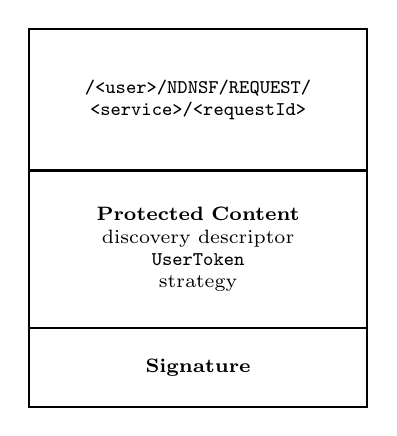
\begin{tikzpicture}[font=\scriptsize, every node/.style={align=center}]
  \draw[thick] (-2.15,2.45) rectangle (2.15,-2.35);
  \draw[thick] (-2.15,0.65) -- (2.15,0.65);
  \draw[thick] (-2.15,-1.35) -- (2.15,-1.35);
  \node[text width=3.9cm] at (0,1.55)
    {\texttt{/<user>/NDNSF/REQUEST/}\\\texttt{<service>/<requestId>}};
  \node[text width=3.8cm] at (0,-0.35)
    {\textbf{Protected Content}\\discovery descriptor\\\texttt{UserToken}\\strategy};
  \node at (0,-1.85) {\textbf{Signature}};
\end{tikzpicture}
\end{center}
\end{columns}
\end{frame}
\fi

\ifshortdeck
\begin{frame}{Runtime Provider Discovery and Selection}
\vspace{-0.12cm}
\begin{center}
\resizebox{0.92\linewidth}{!}{%
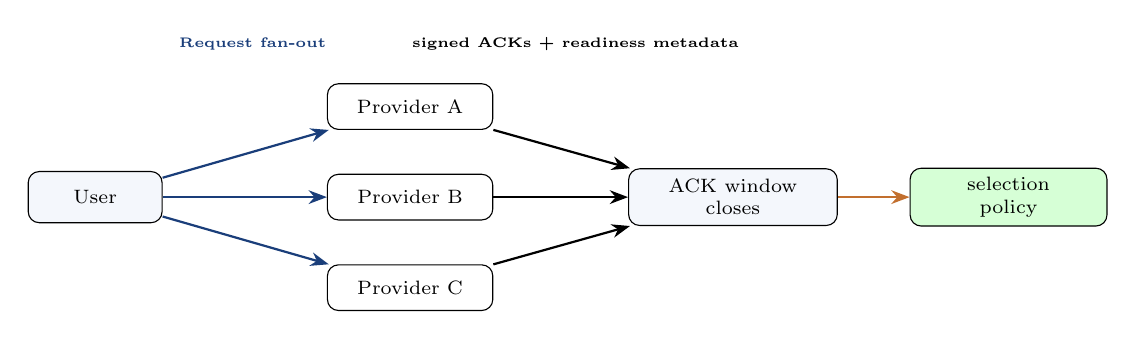
\begin{tikzpicture}[font=\scriptsize, every node/.style={align=center}]
  \node[draw, rounded corners, fill=LightBand, minimum width=1.7cm,
        minimum height=0.65cm] (u) at (0,0) {User};
  \node[draw, rounded corners, fill=white, minimum width=2.1cm,
        minimum height=0.58cm] (p1) at (4.0,1.15) {Provider A};
  \node[draw, rounded corners, fill=white, minimum width=2.1cm,
        minimum height=0.58cm] (p2) at (4.0,0) {Provider B};
  \node[draw, rounded corners, fill=white, minimum width=2.1cm,
        minimum height=0.58cm] (p3) at (4.0,-1.15) {Provider C};
  \node[draw, rounded corners, fill=LightBand, minimum width=2.65cm,
        minimum height=0.72cm] (w) at (8.1,0) {ACK window\\closes};
  \node[draw, rounded corners, fill=green!16, minimum width=2.5cm,
        minimum height=0.72cm] (s) at (11.6,0) {selection\\policy};
  \node[font=\tiny\bfseries, MemphisBlue] at (2.0,1.95) {Request fan-out};
  \node[font=\tiny\bfseries] at (6.1,1.95) {signed ACKs + readiness metadata};
  \foreach \p in {p1,p2,p3} {
    \draw[-{Stealth}, thick, MemphisBlue] (u) -- (\p);
    \draw[-{Stealth}, thick] (\p) -- (w);
  }
  \draw[-{Stealth}, thick, AccentOrange] (w) -- (s);
\end{tikzpicture}%
}
\end{center}

\vspace{0.05cm}
\small
\begin{itemize}
  \item Each Provider evaluates local readiness and may report load, wait time,
        capability, location, model availability, or safety state.
  \item After the ACK collection window closes, the User applies First
        Responding, Random, All Selected, or a custom policy.
  \item Selection authorizes the chosen Provider or Providers to execute.
\end{itemize}
\vspace{0.05cm}
\bluebox{\scriptsize Discovery asks who is willing and capable now; selection decides who should execute.}
\end{frame}
\else
\begin{frame}{Selective ACK}
\textbf{In the normal discovery path, every Provider returns an ACK.}

\vspace{0.45cm}
\begin{columns}[T,onlytextwidth]
\column{0.50\linewidth}
\begin{itemize}
  \item \textbf{Positive ACK:} the Provider is willing and currently capable.
  \item \textbf{Negative ACK:} the Provider received the request but is not ready
        or cannot serve it now.
  \item ACK metadata can report load, wait time, location, model availability, or safety state.
  \item User selects only among Providers with positive ACKs.
\end{itemize}

\column{0.46\linewidth}
\begin{center}
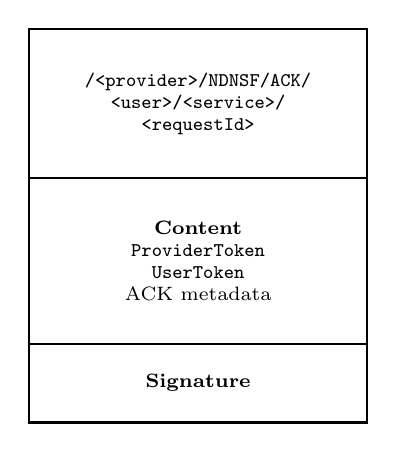
\begin{tikzpicture}[font=\scriptsize, every node/.style={align=center}]
  \draw[thick] (-2.15,2.55) rectangle (2.15,-2.45);
  \draw[thick] (-2.15,0.65) -- (2.15,0.65);
  \draw[thick] (-2.15,-1.45) -- (2.15,-1.45);
  \node[text width=3.95cm] at (0,1.60)
    {\texttt{/<provider>/NDNSF/ACK/}\\
     \texttt{<user>/<service>/}\\
     \texttt{<requestId>}};
  \node[text width=3.8cm] at (0,-0.40)
    {\textbf{Content}\\\texttt{ProviderToken}\\\texttt{UserToken}\\ACK metadata};
  \node at (0,-1.95) {\textbf{Signature}};
\end{tikzpicture}
\end{center}
\end{columns}
\end{frame}

\begin{frame}{Custom Provider Selection Strategy}
\textbf{Provider selection is user-side, policy-driven, and performed after ACK collection.}

\vspace{0.45cm}
\begin{columns}[T,onlytextwidth]
\column{0.50\linewidth}
\begin{itemize}
  \item User collects all ACKs during an ACK window; only positive ACKs become
        selection candidates.
  \item Built-in choices: first responding, random, all selected.
  \item Custom policy can use latency, load, capability, location, or safety metadata.
\end{itemize}

\column{0.46\linewidth}
\begin{center}
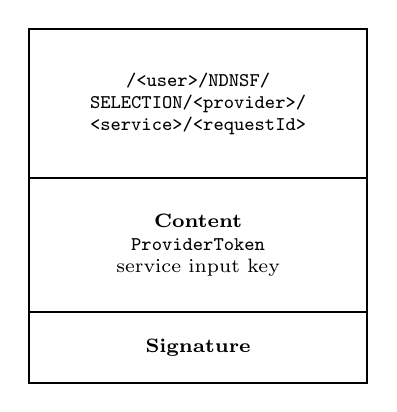
\begin{tikzpicture}[font=\scriptsize, every node/.style={align=center}]
  \draw[thick] (-2.15,2.35) rectangle (2.15,-2.15);
  \draw[thick] (-2.15,0.45) -- (2.15,0.45);
  \draw[thick] (-2.15,-1.25) -- (2.15,-1.25);
  \node[text width=3.95cm] at (0,1.40)
    {\texttt{/<user>/NDNSF/}\\
     \texttt{SELECTION/<provider>/}\\
     \texttt{<service>/<requestId>}};
  \node[text width=3.8cm] at (0,-0.40)
    {\textbf{Content}\\\texttt{ProviderToken}\\service input key};
  \node at (0,-1.70) {\textbf{Signature}};
\end{tikzpicture}
\end{center}
\end{columns}

\vspace{0.05cm}
{\scriptsize \textcolor{MemphisBlue}{\textbf{Key point:} ACK publication is common; ACK status reports readiness, and selection uses positive ACKs.}}
\end{frame}

\begin{frame}{Provider Selection Strategies: Built-In Choices}
\begin{center}
\begin{tabular}{cc}
\textbf{\small First Responding} & \textbf{\small Random Selection} \\
\includegraphics[width=0.44\linewidth,height=0.48\textheight,keepaspectratio]{First-Responding.png} &
\includegraphics[width=0.44\linewidth,height=0.48\textheight,keepaspectratio]{Random-Selection.png}
\end{tabular}
\end{center}
\vspace{0.1cm}
\bluebox{\scriptsize The same Request--ACK collection step can feed simple built-in policies: choose the first ready provider or pick randomly among valid ACKs.}
\end{frame}

\begin{frame}{Provider Selection Strategies: Multi-Provider and Custom}
\begin{center}
\begin{tabular}{cc}
\textbf{\small All Responders} & \textbf{\small Custom Selection Strategy} \\
\includegraphics[width=0.44\linewidth,height=0.48\textheight,keepaspectratio]{All-Responders.png} &
\includegraphics[width=0.44\linewidth,height=0.48\textheight,keepaspectratio]{CustomSelectionStrategy.png}
\end{tabular}
\end{center}
\vspace{0.1cm}
\bluebox{\scriptsize Selection can also choose all ready providers for cooperative execution, or use application-defined metadata such as latency, load, capability, location, or safety state.}
\end{frame}
\fi

\ifshortdeck
\else
\begin{frame}{Completed Foundation: NDNSF v0.1}
\begin{columns}[T,onlytextwidth]
\column{0.43\linewidth}
\begin{itemize}
  \item Implemented generic dynamic C++ API
  \item Multi-provider ACK collection
  \item Provider selection strategies
  \item NDN-SVS patch
  \item MiniNDN evaluation
\end{itemize}

\column{0.53\linewidth}
\textbf{Provider API}\\[0.10cm]
\bluebox{\ttfamily\scriptsize
provider.addHandler\textless RequestT, ResponseT\textgreater(\\
\hspace*{0.35cm}serviceName, handler);}

\vspace{0.22cm}
\textbf{User API}\\[0.10cm]
\bluebox{\ttfamily\scriptsize
user.RequestService\textless RequestT, ResponseT\textgreater(\\
\hspace*{0.35cm}providers, serviceName, request,\\
\hspace*{0.35cm}onResponse, onTimeout, timeoutMs,\\
\hspace*{0.35cm}strategy);}
\end{columns}
\vspace{0.35cm}
\bluebox{\small NDNSF v0.1 (commit \texttt{be9421f\ldots}, tree \texttt{c9cc0c\ldots}) is the May 20 repository baseline; role-based dependency collaboration is post-v0.1 work.}
\end{frame}
\fi

\begin{frame}{Baselines Before the Comparison}
\scriptsize
\begin{columns}[T,onlytextwidth]
\column{0.31\linewidth}
\bluebox{\centering\textbf{gRPC} \slideref{17}}
\begin{center}
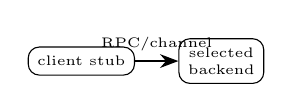
\begin{tikzpicture}[node distance=0.55cm, every node/.style={font=\tiny, align=center}]
  \node[draw, rounded corners] (c) {client stub};
  \node[draw, rounded corners, right=of c] (s) {selected\\backend};
  \draw[-{Stealth}, thick] (c) -- node[above]{RPC/channel} (s);
\end{tikzpicture}
\end{center}
\begin{itemize}
  \item Load balancing chooses among backend addresses supplied beforehand by
        a resolver; it does not discover willing Providers from an RPC.
  \item Here, gRPC-1 uses one endpoint; gRPC-SEQ-4 retries four preregistered endpoints sequentially.
\end{itemize}

\column{0.31\linewidth}
\bluebox{\centering\textbf{NSC} \slideref{10}}
\begin{center}
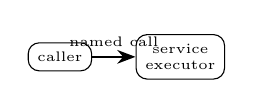
\begin{tikzpicture}[node distance=0.55cm, every node/.style={font=\tiny, align=center}]
  \node[draw, rounded corners] (c) {caller};
  \node[draw, rounded corners, right=of c] (s) {service\\executor};
  \draw[-{Stealth}, thick] (c) -- node[above]{named call} (s);
\end{tikzpicture}
\end{center}
\begin{itemize}
  \item Expresses an RPC-like service call with NDN names.
  \item The evaluated configuration binds one call to one executor.
\end{itemize}

\column{0.34\linewidth}
\bluebox{\centering\textbf{NDNSF}}
\begin{center}
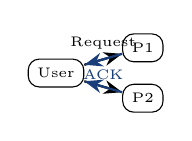
\begin{tikzpicture}[node distance=0.42cm, every node/.style={font=\tiny, align=center}]
  \node[draw, rounded corners] (u) {User};
  \node[draw, rounded corners, right=0.48cm of u, yshift=0.32cm] (p1) {P1};
  \node[draw, rounded corners, right=0.48cm of u, yshift=-0.32cm] (p2) {P2};
  \draw[-{Stealth}, thick] (u) -- node[above]{Request} (p1);
  \draw[-{Stealth}, thick] (u) -- (p2);
  \draw[-{Stealth}, thick, MemphisBlue] (p1) -- node[below]{ACK} (u);
  \draw[-{Stealth}, thick, MemphisBlue] (p2) -- (u);
\end{tikzpicture}
\end{center}
\begin{itemize}
  \item Discovers multiple ready Providers through one ACK window.
  \item Selects after observing runtime willingness and metadata.
\end{itemize}
\end{columns}

\vspace{-0.10cm}
\bluebox{\scriptsize \textbf{Context only:} NDNSF uses submitted v0.1 measurements; NSC/gRPC use one new run per loss with the shown workload and deadline. Batches and semantics differ; no variance or significance claim is made.}
\end{frame}

\ifshortdeck
\begin{frame}{v0.1 Evidence: Network and Provider Failures}
\scriptsize
\begin{columns}[T,onlytextwidth]
\column{0.47\linewidth}
\textbf{Contextual network-loss comparison}
\begin{center}
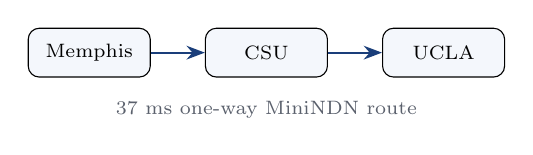
\begin{tikzpicture}[every node/.style={font=\scriptsize, align=center}]
  \tikzset{
    site/.style={draw, rounded corners, fill=LightBand, minimum width=1.55cm, minimum height=0.62cm},
    path/.style={-{Stealth}, thick, MemphisBlue}
  }
  \node[site] (memphis) at (-2.25,0) {Memphis};
  \node[site] (csu) at (0,0) {CSU};
  \node[site] (ucla) at (2.25,0) {UCLA};
  \draw[path] (memphis) -- (csu);
  \draw[path] (csu) -- (ucla);
  \node[SoftGray] at (0,-0.72) {37 ms one-way MiniNDN route};
\end{tikzpicture}
\end{center}
\begin{itemize}
  \item Memphis $\rightarrow$ CSU $\rightarrow$ UCLA; 5\,ms service delay.
  \item 10\,RPS; 5\,s warmup; 60\,s measured; 5\,s deadline.
\end{itemize}
\vspace{0.05cm}
\centering
{\scriptsize
\setlength{\tabcolsep}{2pt}
\begin{tabular}{lrrr}
\toprule
\textbf{Success (\%)} & \textbf{1\%} & \textbf{3\%} & \textbf{10\%}\\
\midrule
\textbf{NDNSF v0.1} & 99.83 & 99.67 & 89.83\\
NSC & 90.17 & 74.00 & 34.67\\
gRPC & 100.00 & 100.00 & 90.17\\
\bottomrule
\end{tabular}
}

\column{0.50\linewidth}
\textbf{Intermittent Provider failures}
\begin{itemize}
  \item Providers reject or disappear with 10--30\% probability.
  \item NDNSF selects among Providers that returned valid ACKs.
\end{itemize}
\vspace{0.15cm}
\centering
\begin{tabular}{lrrr}
\toprule
\textbf{System} & \textbf{10\%} & \textbf{20\%} & \textbf{30\%}\\
\midrule
NSC & 83.25 & 66.58 & 49.92\\
gRPC & 83.35 & 66.69 & 65.36\\
\textbf{NDNSF} & \textbf{99.82} & \textbf{99.46} & \textbf{96.70}\\
\bottomrule
\end{tabular}
\end{columns}

\vspace{0.16cm}
\bluebox{\scriptsize \textbf{Context only:} NDNSF uses submitted v0.1 results; NSC/gRPC use one new run per loss. Batches and Provider-selection semantics differ; no variance or significance claim is made.}
\end{frame}

\begin{frame}{Four-Provider Mobility Holdout}
\scriptsize
\begin{center}
\includegraphics[width=0.96\linewidth,height=0.50\textheight,keepaspectratio]{assets/mobility_seed_repeat_followup.png}
\end{center}
\vspace{-0.05cm}
\begin{columns}[T,onlytextwidth]
\column{0.47\linewidth}
\bluebox{\tiny \textbf{Follow-up:} same one AP/four-Provider condition,
50\,m/2\,m/s, new seeds 50--59, same 4\,s barrier, 60\,s at 5 RPS,
1\,s attempt/ACK, 5\,s deadline, admission and health routing off.}
\column{0.47\linewidth}
\bluebox{\tiny \textbf{Result:} NDNSF 74.50\%; gRPC-SEQ-4 74.10\%;
NSC-4 72.47\%. NDNSF$-$gRPC is $+0.40$ pp, 95\% CI
$[-0.03,+0.97]$ pp; the gate is not met.}
\end{columns}
\end{frame}
\else
\begin{frame}{Network Loss: NDNSF v0.1 and Baselines}
\scriptsize
\begin{columns}[T,onlytextwidth]
\column{0.43\linewidth}
\textbf{Common topology and workload}
\begin{center}
\includegraphics[width=0.98\linewidth,height=0.47\textheight,keepaspectratio]{assets/testbed_topo.png}
\end{center}
\vspace{-0.22cm}
{\tiny
\textbf{Path:} Memphis $\rightarrow$ CSU $\rightarrow$ UCLA; 37\,ms one way.\\[0.05cm]
\textbf{Load:} 10\,RPS; 5\,ms service delay; 1/3/10\% per-link loss.\\[0.05cm]
\textbf{NDNSF run:} 60\,s after warmup; 600 measured requests.
}

\column{0.55\linewidth}
\textbf{Service success rate (\%)}\\[-0.05cm]
{\tiny Submitted NDNSF v0.1 values (10\%: best measured); new NSC/gRPC: one run per loss. Configuration-aligned context only; no variance or significance claim.}

\vspace{-0.02cm}
\begin{center}
\includegraphics[width=\linewidth,height=0.47\textheight,keepaspectratio]{assets/page30_network_loss_chart.png}
\end{center}
\end{columns}

\vspace{-0.02cm}
\bluebox{\tiny \textbf{Result:} With SVS retry, NDNSF completed 599/600, 598/600, and 539/600 requests at 1\%, 3\%, and 10\% link loss.}
\end{frame}

\begin{frame}{Historical v0.1: Provider Failures}
\scriptsize
\begin{columns}[T,onlytextwidth]
\column{0.44\linewidth}
\textbf{Historical experiment}
\begin{itemize}
  \item Memphis User; identical service Providers at UCLA, WUSTL, and UIUC.
  \item Every 10 s, each Provider independently starts a 10 s rejection period with probability 10/20/30\%.
  \item Unavailable NDNSF Providers suppress ACKs; FirstResponding selects a valid candidate.
  \item NSC and gRPC use one fixed target and no failover.
\end{itemize}

\vspace{0.08cm}
\textbf{What this established}
\begin{itemize}
  \item NDNSF remains above 96\% success at the 30\% setting.
  \item Motivation only; not a matched failover comparison.
\end{itemize}

\column{0.53\linewidth}
\centering
{\footnotesize\textbf{Historical multi-provider topology}}\\[0.10cm]

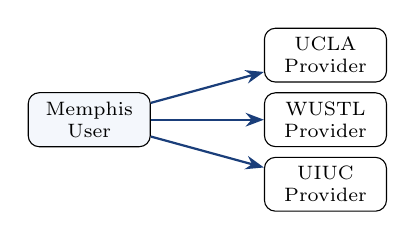
\begin{tikzpicture}[x=1cm,y=1cm, every node/.style={font=\scriptsize, align=center}]
  \node[draw, rounded corners, fill=LightBand, minimum width=1.55cm,
        minimum height=0.58cm] (u) at (0,0) {Memphis\\User};
  \node[draw, rounded corners, fill=white, minimum width=1.55cm,
        minimum height=0.58cm] (p1) at (3.0,0.82) {UCLA\\Provider};
  \node[draw, rounded corners, fill=white, minimum width=1.55cm,
        minimum height=0.58cm] (p2) at (3.0,0) {WUSTL\\Provider};
  \node[draw, rounded corners, fill=white, minimum width=1.55cm,
        minimum height=0.58cm] (p3) at (3.0,-0.82) {UIUC\\Provider};
  \draw[-{Stealth}, thick, MemphisBlue] (u) -- (p1);
  \draw[-{Stealth}, thick, MemphisBlue] (u) -- (p2);
  \draw[-{Stealth}, thick, MemphisBlue] (u) -- (p3);
\end{tikzpicture}

\vspace{0.04cm}

{\footnotesize\textbf{Request success rate (\%)}}\\[0.18cm]
\begingroup
\footnotesize
\setlength{\tabcolsep}{8pt}
\renewcommand{\arraystretch}{1.25}
\begin{tabular}{lrrr}
\toprule
\textbf{System} & \textbf{10\%} & \textbf{20\%} & \textbf{30\%}\\
\midrule
NSC & 83.25 & 66.58 & 49.92\\
gRPC & 83.35 & 66.69 & 65.36\\
\textbf{NDNSF} & \textbf{99.82} & \textbf{99.46} & \textbf{96.70}\\
\bottomrule
\end{tabular}
\endgroup

\end{columns}

\vspace{0.04cm}
\bluebox{\tiny \textbf{Evidence boundary:} historical configuration-level result; the baselines are not the four-target sequential clients evaluated on Slides 32--33.}
\end{frame}

\begin{frame}{Four-Provider Mobility: Experiment Design}
\scriptsize
\begin{columns}[T,onlytextwidth]
\column{0.43\linewidth}
\textbf{One-AP field and evaluated radii}
\begin{center}
\includegraphics[width=0.94\linewidth,height=0.54\textheight,keepaspectratio]{assets/mobility_topology_50_100_150m_2ms.png}
\end{center}
\bluebox{\tiny 400\,$\times$\,400\,m field; AP at (200,200); 2\,m/s random waypoint;
300\,s simulated burn-in.}

\column{0.54\linewidth}
\textbf{Matched systems and controls}
\vspace{0.02cm}
\renewcommand{\arraystretch}{1.02}
\setlength{\tabcolsep}{3pt}
\begin{tabular}{>{\raggedright\arraybackslash}p{0.25\linewidth}>{\raggedright\arraybackslash}p{0.66\linewidth}}
\toprule
\textbf{System} & \textbf{Client behavior}\\
\midrule
\textbf{NDNSF} & runtime ACKs; FirstResponding + bounded reselection\\
gRPC-SEQ-4 & four registered IPs; sequential 1\,s retry\\
NSC-4 & four registered prefixes; sequential 1\,s retry\\
\bottomrule
\end{tabular}

\vspace{0.08cm}
\textbf{Two matched analysis layers}
\begin{itemize}\setlength{\itemsep}{0pt}\setlength{\parskip}{0pt}
  \item \textbf{All requests:} 50/100/150\,m; coverage control.
  \item \textbf{Independent switching test:} 100\,m; actual publication time
        and applied-gate agreement.
  \item 5 RPS, 60\,s; 1\,s attempt/ACK; 5\,s deadline; admission and health
        routing disabled.
  \item \texttt{block\_network=true}; same trace; 4.05\,s request phase.
\end{itemize}
\bluebox{\tiny NDNSF does not require a pre-registered Provider endpoint list;
gRPC and NSC receive the same four targets before each run.}
\end{columns}
\end{frame}

\begin{frame}{Mobility Results: Coverage and Switching}
\scriptsize
\vspace{0.12cm}
\begin{center}
\includegraphics[width=0.96\linewidth,height=0.53\textheight,keepaspectratio]{assets/mobility_burnin_10seed_results.png}
\end{center}
\vspace{-0.02cm}
\begin{columns}[T,onlytextwidth]
\column{0.48\linewidth}
\bluebox{\tiny \textbf{All requests:} At 50\,m, all systems succeed on only
about 54--55\% of requests. At 100\,m, success is about 98\%; at 150\,m, it
reaches 100\%. The main driver is which Providers are actually covered when a
request is published.}
\column{0.48\linewidth}
\bluebox{\tiny \textbf{When switching is needed:} Among 1,312 matched requests
where the initial Provider was unavailable but another Provider was reachable,
NDNSF's tail latency was 597\,ms lower than gRPC and 2.62\,s lower than NSC.
The intervals are shown in the chart. Success rates were
99.92/98.86/98.78\% for NDNSF/gRPC/NSC; no overall success-rate advantage is
claimed: actual Provider coverage at publication time dominates success.}
\end{columns}
\end{frame}

\begin{frame}{NDNSF v0.1 Evaluation: Availability}
\scriptsize
\begin{columns}[T,onlytextwidth]
\column{0.45\linewidth}
\textbf{Experiment settings}
\begin{itemize}
  \item Real-machine test: Odroid User with laptop and PC Providers.
  \item The laptop is unavailable during the first half; the PC is unavailable
        during the middle half.
  \item Their unavailable windows overlap for one quarter of the run.
\end{itemize}

\vspace{0.22cm}
\textbf{Observation}
\begin{itemize}\setlength{\itemsep}{0pt}
  \item At least one Provider is available for 75\% of the run. This is the
        provider-time coverage ceiling, not a guaranteed success rate.
  \item NDNSF reaches 74.62\% at 10 RPS and 73.73\% at 30 RPS.
  \item The small gap below 75\% is failover delay: an in-flight request can
        hit its deadline before another Provider is selected.
  \item SVS/Sync retransmission recovers lost Data, not Provider outages;
        recovery after the deadline still fails.
\end{itemize}

\column{0.52\linewidth}
\centering
\textbf{Provider availability over time}
\vspace{0.08cm}

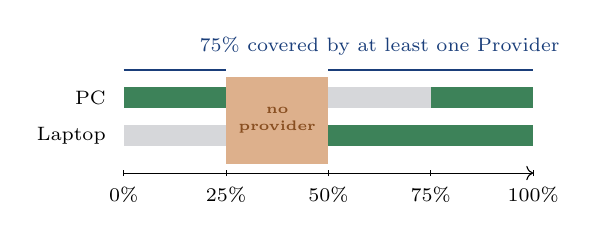
\begin{tikzpicture}[x=0.052cm,y=0.48cm, every node/.style={font=\scriptsize}]
  \draw[->] (0,0) -- (100,0);
  \foreach \x/\lab in {0/0\%,25/25\%,50/50\%,75/75\%,100/100\%} {
    \draw (\x,-0.08) -- (\x,0.08);
    \node[anchor=north] at (\x,-0.12) {\lab};
  }
  \node[anchor=east] at (-2,1.0) {Laptop};
  \node[anchor=east] at (-2,2.0) {PC};
  \fill[SoftGray!25] (0,0.72) rectangle (50,1.28);
  \fill[AccentGreen] (50,0.72) rectangle (100,1.28);
  \fill[AccentGreen] (0,1.72) rectangle (25,2.28);
  \fill[SoftGray!25] (25,1.72) rectangle (75,2.28);
  \fill[AccentGreen] (75,1.72) rectangle (100,2.28);
  \fill[AccentOrange!55] (25,0.25) rectangle (50,2.55);
  \node[align=center, font=\tiny\bfseries, AccentOrange!70!black] at (37.5,1.4) {no\\provider};
  \draw[MemphisBlue, thick] (0,2.72) -- (25,2.72);
  \draw[MemphisBlue, thick] (50,2.72) -- (100,2.72);
  \node[anchor=south, MemphisBlue] at (62.5,2.86) {75\% covered by at least one Provider};
\end{tikzpicture}

\vspace{0.12cm}
\textbf{Measured request success (not time coverage)}
\vspace{0.03cm}
\includegraphics[width=\linewidth,height=0.28\textheight,keepaspectratio]{assets/TABLE4.png}
\end{columns}
\end{frame}

\begin{frame}{Mobility Evidence: What We Can Claim}
\scriptsize
\begin{columns}[T,onlytextwidth]
\column{0.31\linewidth}
\bluebox{\textbf{Historical v0.1 demonstrations}}
\begin{itemize}
  \item Provider rejection and availability
  \item One NSC/gRPC target
  \item No seed-level inference
  \item \textbf{Role:} motivation only
\end{itemize}

\column{0.31\linewidth}
\bluebox{\textbf{Matched all-request controls}}
\begin{itemize}
  \item Same trace; four targets
  \item 50/100/150\,m; repeated runs
  \item Coverage dominates success
  \item No universal advantage
  \item \textbf{Role:} negative controls
\end{itemize}

\column{0.31\linewidth}
\bluebox{\textbf{Independent switching test}}
\begin{itemize}
  \item 1,312 matched switching requests
  \item Tail latency: 597\,ms below gRPC
  \item Tail latency: 2,618\,ms below NSC
  \item Comparable success
  \item \textbf{Role:} confirmatory evidence
\end{itemize}
\end{columns}

\vspace{0.28cm}
\bluebox{\small \textbf{Supported conclusion:} When a Provider switch is required, runtime discovery reduces tail latency versus sequential retry over pre-registered targets; it is not universally better under mobility.}
\end{frame}
\fi

\begin{frame}{What NDNSF v0.1 Still Lacks}
\small
\begin{columns}[T,onlytextwidth]
\column{0.47\linewidth}
\bluebox{\textbf{Completed v0.1 evidence}}
\begin{itemize}
  \item Runtime discovery and service ACKs reporting willingness and status
  \item Provider selection under failure and mobility
  \item Request-level authorization and token binding
\end{itemize}

\column{0.50\linewidth}
\bluebox{\textbf{Still missing for collaboration}}
\begin{itemize}
  \item Assign different Providers to different application roles, such as capture, detection, and mapping.
  \item Record which role is allowed to send Data to which downstream role.
  \item Verify that received Data came from the Provider assigned to the authorized preceding role, whether fetched directly or from a cache.
\end{itemize}
\end{columns}

\vspace{0.12cm}
\bluebox{\small UAV and distributed inference are requirement generators: they expose why Provider selection alone is insufficient for multi-role execution.}
\end{frame}

\ifshortdeck
\begin{frame}{UAV Workload and Requirements}
\begin{columns}[T,onlytextwidth]
\column{0.54\linewidth}
\begin{center}
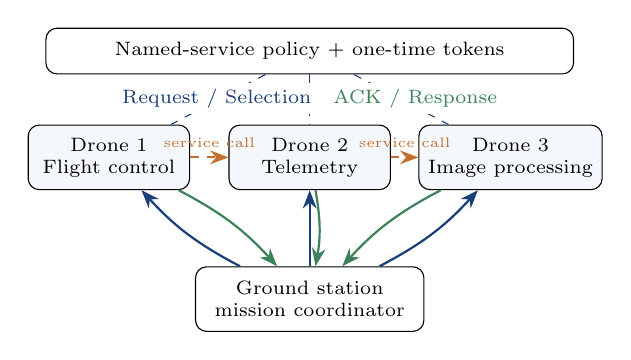
\begin{tikzpicture}[every node/.style={font=\scriptsize, align=center}]
\tikzset{
  drone/.style={draw, rounded corners, fill=LightBand, minimum width=2.05cm, minimum height=0.82cm},
  ground/.style={draw, rounded corners, fill=white, minimum width=2.9cm, minimum height=0.82cm},
  flow/.style={-{Stealth}, thick, MemphisBlue},
  return/.style={-{Stealth}, thick, AccentGreen}
}
  \node[draw, rounded corners, fill=white, minimum width=6.7cm, minimum height=0.58cm] (policy) at (0,2.0)
    {Named-service policy + one-time tokens};
  \node[drone] (d1) at (-2.55,0.65) {Drone 1\\Flight control};
  \node[drone] (d2) at (0,0.65) {Drone 2\\Telemetry};
  \node[drone] (d3) at (2.55,0.65) {Drone 3\\Image processing};
  \node[ground] (gs) at (0,-1.15) {Ground station\\mission coordinator};
  \draw[flow] (gs) to[bend left=10] (d1);
  \draw[return] (d1) to[bend left=10] (gs);
  \draw[flow] (gs) -- (d2);
  \draw[return] (d2) to[bend left=10] (gs);
  \draw[flow] (gs) to[bend right=10] (d3);
  \draw[return] (d3) to[bend right=10] (gs);
  \draw[-{Stealth}, dashed, thick, AccentOrange] (d1) -- node[above, font=\tiny]{service call} (d2);
  \draw[-{Stealth}, dashed, thick, AccentOrange] (d2) -- node[above, font=\tiny]{service call} (d3);
  \draw[dashed, MemphisBlue] (policy) -- (d1);
  \draw[dashed, MemphisBlue] (policy) -- (d2);
  \draw[dashed, MemphisBlue] (policy) -- (d3);
  \node[fill=white, inner sep=2pt] at (0,1.40)
    {\textcolor{MemphisBlue}{Request / Selection}\quad
     \textcolor{AccentGreen}{ACK / Response}};
\end{tikzpicture}
\end{center}

\column{0.43\linewidth}
\small
\begin{itemize}
  \item Mobility and changing reachability
  \item Command authorization
  \item Telemetry freshness
  \item Video and recording objects
  \item Multi-drone missions
\end{itemize}
\end{columns}
\vspace{0.16cm}
\bluebox{\scriptsize The ground station and drones may all invoke services; each drone can act as both an NDNSF User and Provider during a mission.}
\end{frame}
\else
\begin{frame}{UAV Workload}
\begin{center}
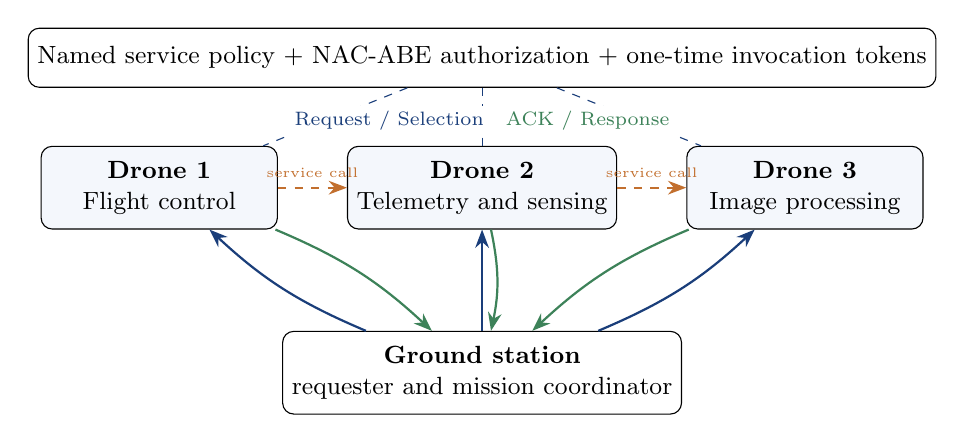
\begin{tikzpicture}[x=1cm,y=1cm, every node/.style={font=\small, align=center}]
\tikzset{
  drone/.style={draw, rounded corners, fill=LightBand, minimum width=3.0cm, minimum height=1.05cm},
  ground/.style={draw, rounded corners, fill=white, minimum width=3.5cm, minimum height=1.05cm},
  flow/.style={-{Stealth}, thick, MemphisBlue},
  return/.style={-{Stealth}, thick, AccentGreen}
}
  \node[draw, rounded corners, fill=white, minimum width=8.8cm, minimum height=0.75cm] (policy) at (0,2.55)
    {Named service policy + NAC-ABE authorization + one-time invocation tokens};
  \node[drone] (d1) at (-4.1,0.90) {\textbf{Drone 1}\\Flight control};
  \node[drone] (d2) at (0,0.90) {\textbf{Drone 2}\\Telemetry and sensing};
  \node[drone] (d3) at (4.1,0.90) {\textbf{Drone 3}\\Image processing};
  \node[ground] (gs) at (0,-1.45) {\textbf{Ground station}\\requester and mission coordinator};

  \draw[flow] (gs) to[bend left=10] (d1);
  \draw[return] (d1) to[bend left=10] (gs);
  \draw[flow] (gs) -- (d2);
  \draw[return] (d2) to[bend left=12] (gs);
  \draw[flow] (gs) to[bend right=10] (d3);
  \draw[return] (d3) to[bend right=10] (gs);
  \draw[-{Stealth}, dashed, thick, AccentOrange] (d1) -- node[above, font=\tiny]{service call} (d2);
  \draw[-{Stealth}, dashed, thick, AccentOrange] (d2) -- node[above, font=\tiny]{service call} (d3);
  \draw[dashed, MemphisBlue] (policy) -- (d1);
  \draw[dashed, MemphisBlue] (policy) -- (d2);
  \draw[dashed, MemphisBlue] (policy) -- (d3);
  \node[fill=white, inner sep=2pt, font=\scriptsize] at (0,1.75)
    {\textcolor{MemphisBlue}{Request / Selection}\quad
     \textcolor{AccentGreen}{ACK / Response}};
\end{tikzpicture}
\end{center}
\bluebox{The ground station and drones may all invoke services; each drone can act as both an NDNSF User and Provider during a mission.}
\end{frame}

\begin{frame}{Requirements of a UAV Network Application}
\begin{itemize}
  \item Mobility and changing reachability
  \item Command authorization
  \item Telemetry freshness
  \item Video and recording objects
  \item Multi-drone missions
\end{itemize}
\bluebox{This dissertation will not produce a comprehensive UAV application. Instead, it will develop the NDNSF mechanisms needed to support this class of application.}
\end{frame}
\fi

\begin{frame}{UAV Requirements $\rightarrow$ NDNSF Mechanisms}
\footnotesize
\begin{tabularx}{\linewidth}{>{\raggedright\arraybackslash}p{0.31\linewidth}>{\raggedright\arraybackslash}X}
\toprule
\textbf{UAV requirement} & \textbf{NDNSF mechanism}\\
\midrule
Mobility and changing reachability &
Service ACKs report willingness and runtime status; NDNSF selects a responding Provider. Optional bounded response reselection may run after selection.\\
\midrule
Command authorization &
Targeted invocation with NAC-ABE, one-time tokens, and replay checks\\
\midrule
Telemetry freshness &
Versioned names, freshness/expiry checks, and lifecycle state\\
\midrule
Video and recording objects &
Immutable object references, manifests, and segmented cache/Repo retrieval\\
\midrule
Multi-drone missions &
Assign Providers to mission roles; accept Data only from the Provider assigned to the authorized preceding role.\\
\bottomrule
\end{tabularx}

\vspace{0.12cm}
\bluebox{\scriptsize Generic one-to-many calls use ACK and Selection. Targeted calls skip them only after a Provider/service token batch has been bootstrapped.}
\end{frame}

\ifshortdeck
\begin{frame}{Distributed Inference Motivation and Challenge}
\begin{columns}[T,onlytextwidth]
\column{0.47\linewidth}
\begin{center}
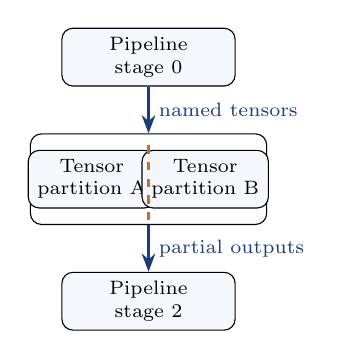
\begin{tikzpicture}[x=1cm,y=1cm, every node/.style={font=\scriptsize, align=center}]
  \node[draw, rounded corners, fill=LightBand, minimum width=2.2cm,
        minimum height=0.72cm] (s0) at (0,1.55) {Pipeline\\stage 0};
  \node[draw, rounded corners, fill=white, minimum width=3.0cm,
        minimum height=1.15cm] (s1) at (0,0) {};
  \node[draw, rounded corners, fill=LightBand, minimum width=1.15cm,
        minimum height=0.65cm] at (-0.72,0) {Tensor\\partition A};
  \node[draw, rounded corners, fill=LightBand, minimum width=1.15cm,
        minimum height=0.65cm] at (0.72,0) {Tensor\\partition B};
  \node[draw, rounded corners, fill=LightBand, minimum width=2.2cm,
        minimum height=0.72cm] (s2) at (0,-1.55) {Pipeline\\stage 2};
  \draw[-{Stealth}, thick, MemphisBlue] (s0) -- node[right]{named tensors} (s1);
  \draw[-{Stealth}, thick, MemphisBlue] (s1) -- node[right]{partial outputs} (s2);
  \draw[dashed, AccentOrange, thick] (0,-0.52) -- (0,0.52);
\end{tikzpicture}
\end{center}

\column{0.50\linewidth}
\small
\textbf{One run must align}
\begin{itemize}
  \item canonical model layers,
  \item pipeline stages and tensor partitions,
  \item Provider and device assignments,
  \item named dependencies and collectives.
\end{itemize}
\vspace{0.18cm}
\textbf{Why it matters:} Providers and visible devices are known only after ACK collection, yet every stage must assemble and consume the correct data.
\end{columns}
\vspace{0.16cm}
\bluebox{\scriptsize DI stresses the central problem: turn runtime Provider capabilities into a verified pipeline and tensor execution plan.}
\end{frame}
\else
\begin{frame}{Distributed Inference: Splitting a YOLO Model}
\scriptsize
\begin{columns}[T,onlytextwidth]
\column{0.56\linewidth}
\textbf{Layer-wise (horizontal) cuts: contiguous layer groups form pipeline stages}
\vspace{0.14cm}
\begin{center}
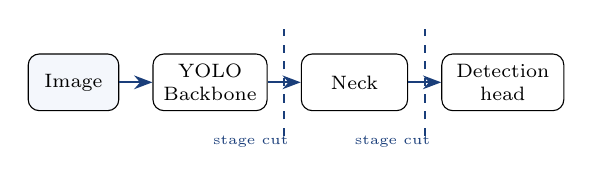
\begin{tikzpicture}[node distance=0.42cm, every node/.style={font=\scriptsize, align=center}]
  \node[draw, rounded corners, fill=LightBand, minimum width=1.15cm,
        minimum height=0.72cm] (in) {Image};
  \node[draw, rounded corners, fill=white, right=of in, minimum width=1.45cm,
        minimum height=0.72cm] (bb) {YOLO\\Backbone};
  \node[draw, rounded corners, fill=white, right=of bb, minimum width=1.35cm,
        minimum height=0.72cm] (neck) {Neck};
  \node[draw, rounded corners, fill=white, right=of neck, minimum width=1.55cm,
        minimum height=0.72cm] (head) {Detection\\head};
  \draw[-{Stealth}, thick, MemphisBlue] (in) -- (bb);
  \draw[-{Stealth}, thick, MemphisBlue] (bb) -- (neck);
  \draw[-{Stealth}, thick, MemphisBlue] (neck) -- (head);
  \draw[dashed, MemphisBlue, thick] ($(bb.east)!0.5!(neck.west)+(0,-0.68)$) --
    ($(bb.east)!0.5!(neck.west)+(0,0.68)$);
  \draw[dashed, MemphisBlue, thick] ($(neck.east)!0.5!(head.west)+(0,-0.68)$) --
    ($(neck.east)!0.5!(head.west)+(0,0.68)$);
  \node[font=\tiny, MemphisBlue] at (2.25,-0.75) {stage cut};
  \node[font=\tiny, MemphisBlue] at (4.05,-0.75) {stage cut};
\end{tikzpicture}
\end{center}
\vspace{0.20cm}
Each stage owns a contiguous layer range and sends named intermediate activations to the next stage.

\column{0.41\linewidth}
\textbf{Tensor-wise (vertical) cut: one layer or stage is partitioned across devices}
\vspace{0.14cm}
\begin{center}
  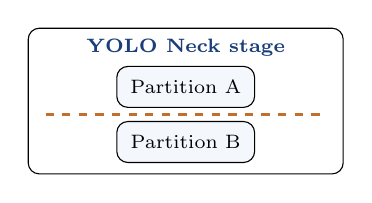
\begin{tikzpicture}[every node/.style={font=\scriptsize, align=center}]
  \node[draw, rounded corners, fill=white, minimum width=4.0cm,
        minimum height=1.85cm] (stage) at (0,0) {};
  \node[font=\scriptsize\bfseries, MemphisBlue] at (0,0.68) {YOLO Neck stage};
  \node[draw, rounded corners, fill=LightBand, minimum width=1.75cm,
        minimum height=0.52cm] at (0,0.18) {Partition A};
  \node[draw, rounded corners, fill=LightBand, minimum width=1.75cm,
        minimum height=0.52cm] at (0,-0.52) {Partition B};
  \draw[dashed, AccentOrange, thick] (-1.78,-0.17) -- (1.78,-0.17);
\end{tikzpicture}
\end{center}
\vspace{0.20cm}
Each partition computes a slice of the same layer or stage; partial outputs may require exchange or aggregation.
\end{columns}

\vspace{0.22cm}
\bluebox{\scriptsize A hybrid layout combines layer-wise pipeline cuts with tensor-wise partitions; NDNSF assigns each stage or partition and device to the selected Providers.}
\end{frame}

\begin{frame}{Distributed Inference Challenge}
\scriptsize
\begin{columns}[T,onlytextwidth]
\column{0.38\linewidth}
\textbf{Information available for one YOLO request}
\begin{itemize}
  \item signed NDN Data objects containing reusable YOLO layer artifacts;
  \item ONNX Runtime plus an NDNSF-DI adapter that interprets and splits the model;
  \item Provider offers describing CPU/GPU, memory, load, and cached layers;
  \item the input image and deadline.
\end{itemize}

\column{0.59\linewidth}
\textbf{Example collaboration plan}
\vspace{0.12cm}
\begin{center}
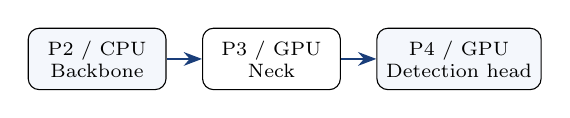
\begin{tikzpicture}[node distance=0.45cm, every node/.style={font=\scriptsize, align=center}]
  \node[draw, rounded corners, fill=LightBand, minimum width=1.75cm,
        minimum height=0.78cm] (p2) {P2 / CPU\\Backbone};
  \node[draw, rounded corners, fill=white, right=of p2, minimum width=1.75cm,
        minimum height=0.78cm] (p3) {P3 / GPU\\Neck};
  \node[draw, rounded corners, fill=LightBand, right=of p3, minimum width=1.75cm,
        minimum height=0.78cm] (p4) {P4 / GPU\\Detection head};
  \draw[-{Stealth}, thick, MemphisBlue] (p2) -- (p3);
  \draw[-{Stealth}, thick, MemphisBlue] (p3) -- (p4);
\end{tikzpicture}
\end{center}

\begin{itemize}
  \item P2, P3, and P4 receive only their assigned model parts and device instructions.
  \item Named intermediate tensors connect the assigned roles; each pipeline stage is a DI role.
  \item The plan is fixed only after signed Provider offers are collected.
\end{itemize}
\end{columns}
\vspace{0.14cm}
\bluebox{\scriptsize A proposed collaboration plan states which Provider runs each role, on which device, with which model part, and which Data may flow to the downstream role.}
\end{frame}
\fi

\begin{frame}{DI Requirements $\rightarrow$ Proposed NDNSF-DI Mechanisms}
\scriptsize
\setlength{\tabcolsep}{3pt}
\renewcommand{\arraystretch}{1.00}
\begin{tabularx}{\linewidth}{>{\raggedright\arraybackslash}p{0.36\linewidth}>{\raggedright\arraybackslash}X}
\toprule
\textbf{Distributed-inference requirement} & \textbf{NDNSF mechanism}\\
\midrule
Run a model that does not fit on one available device &
Split the model into pipeline stages and, where supported, parallel tensor partitions\\
\midrule
Use heterogeneous CPU and GPU Providers effectively &
Collect signed Provider offers, then choose Providers and devices after the ACK window closes\\
\midrule
Avoid copying a complete model for every request &
Reuse signed layer artifacts from an NDN Repo or cache; each Provider prepares only its assigned model part\\
\midrule
Send intermediate tensors only along the planned pipeline &
Assign Providers to roles and verify each tensor's request, signer, preceding role, and name\\
\midrule
Continue when a selected Provider becomes unavailable &
Use authenticated status and bounded replanning or Provider reselection within the request deadline\\
\bottomrule
\end{tabularx}

\vspace{0.14cm}
\bluebox{\scriptsize NDNSF carries Request, ACK, Selection, and Data. Proposed NDNSF-DI mechanisms interpret the model, choose the split, assign devices, and run each model part.}
\end{frame}

\begin{frame}{Post-v0.1: From Application Roles to an Execution Plan}
\scriptsize
\begin{columns}[T,onlytextwidth]
\column{0.61\linewidth}
\begin{center}
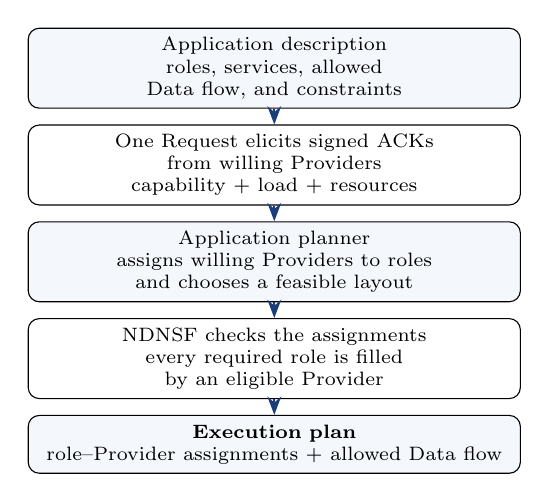
\begin{tikzpicture}[node distance=0.20cm, every node/.style={font=\scriptsize, align=center}]
  \node[draw, rounded corners, fill=LightBand, text width=6.0cm,
        minimum width=6.25cm, minimum height=0.58cm] (template)
    {Application description\\roles, services, allowed Data flow, and constraints};
  \node[draw, rounded corners, fill=white, below=of template, text width=6.0cm,
        minimum width=6.25cm, minimum height=0.58cm] (acks)
    {One Request elicits signed ACKs\\from willing Providers\\capability + load + resources};
  \node[draw, rounded corners, fill=LightBand, below=of acks, text width=6.0cm,
        minimum width=6.25cm, minimum height=0.58cm] (planner)
    {Application planner\\assigns willing Providers to roles and chooses a feasible layout};
  \node[draw, rounded corners, fill=white, below=of planner, text width=6.0cm,
        minimum width=6.25cm, minimum height=0.58cm] (validator)
    {NDNSF checks the assignments\\every required role is filled by an eligible Provider};
  \node[draw, rounded corners, fill=LightBand, below=of validator, text width=6.0cm,
        minimum width=6.25cm, minimum height=0.58cm] (plan)
    {\textbf{Execution plan}\\role--Provider assignments + allowed Data flow};
  \foreach \x/\y in {template/acks,acks/planner,planner/validator,validator/plan}
    \draw[-{Stealth}, thick, MemphisBlue] (\x) -- (\y);
\end{tikzpicture}
\end{center}

\column{0.36\linewidth}
\textbf{Example after ACK collection}
\vspace{0.10cm}

\begin{tabular}{@{}ll@{}}
\toprule
Role & Provider\\
\midrule
Capture & UAV-1\\
Detection & Edge-2\\
Mapping & GS-1\\
\bottomrule
\end{tabular}

\vspace{0.22cm}
\textbf{Allowed Data flow}
\begin{itemize}
  \item Capture image $\rightarrow$ Detection
  \item Detected objects $\rightarrow$ Mapping
\end{itemize}

\vspace{0.08cm}
\textcolor{MemphisBlue}{Only Providers that returned a valid ACK for this request may be assigned a role.}
\end{columns}
\end{frame}

\begin{frame}{Proposed: Verify Data Between Assigned Roles}
\scriptsize
\begin{columns}[T,onlytextwidth]
\column{0.47\linewidth}
\textbf{YOLO example from the execution plan}

\vspace{0.12cm}
\begin{center}
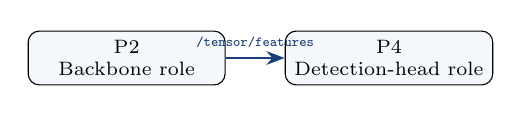
\begin{tikzpicture}[node distance=0.75cm, every node/.style={font=\scriptsize, align=center}]
  \node[draw, rounded corners, fill=LightBand, minimum width=2.5cm] (p2)
    {P2\\Backbone role};
  \node[draw, rounded corners, fill=LightBand, right=of p2, minimum width=2.5cm] (p4)
    {P4\\Detection-head role};
  \draw[-{Stealth}, thick, MemphisBlue] (p2) -- node[above, font=\tiny]
    {\texttt{/tensor/features}} (p4);
\end{tikzpicture}
\end{center}

\textbf{Before P4 processes the tensor, it checks}
\begin{itemize}
  \item it belongs to the current request;
  \item the signer is P2, assigned to Backbone;
  \item Backbone is the allowed preceding role;
  \item its name is under \texttt{/tensor/features}.
\end{itemize}

\column{0.49\linewidth}
\textbf{Expected decisions}
\vspace{0.12cm}
\begin{itemize}
  \item \textcolor{AccentGreen}{\textbf{Accept:}} correctly signed P2 feature tensor.
  \item \textcolor{AccentGreen}{\textbf{Accept:}} the same valid tensor retrieved from an NDN cache.
  \item \textcolor{red!70!black}{\textbf{Reject:}} unassigned P3 uses the same request ID.
  \item \textcolor{red!70!black}{\textbf{Reject:}} P2 publishes on an undeclared Data name.
  \item \textcolor{red!70!black}{\textbf{Reject:}} a valid old tensor is replayed for another request.
\end{itemize}

\vspace{0.16cm}
\bluebox{\scriptsize The proposed Plan-to-Data mechanism turns the execution plan into checks performed by each Provider.}
\end{columns}
\end{frame}

\begin{frame}{Proposed NDNSF-DI Architecture}
\vspace{-0.25cm}
\begin{center}
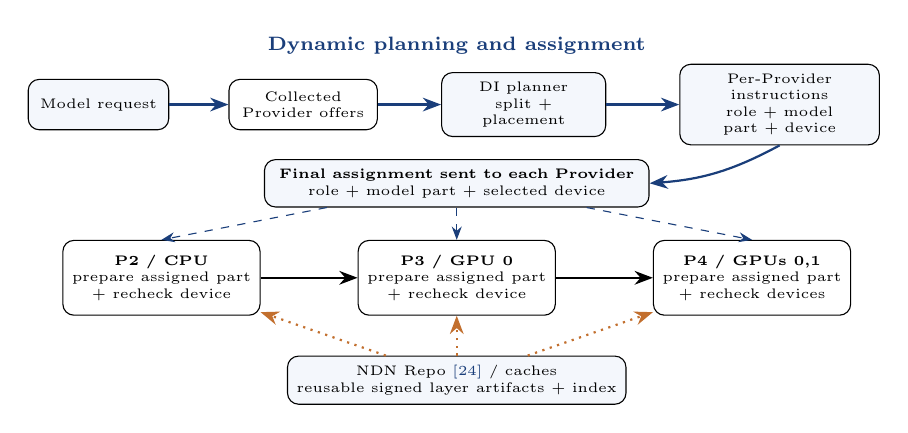
\begin{tikzpicture}[x=1cm,y=1cm, every node/.style={font=\tiny, align=center}]
  \node[font=\scriptsize\bfseries, MemphisBlue] at (5.0,1.70) {Dynamic planning and assignment};
  \node[draw, rounded corners, fill=LightBand, text width=1.55cm, minimum height=0.64cm] (request) at (0.45,0.95) {Model request};
  \node[draw, rounded corners, fill=white, text width=1.65cm, minimum height=0.64cm] (ack) at (3.05,0.95) {Collected Provider offers};
  \node[draw, rounded corners, fill=LightBand, text width=1.85cm, minimum height=0.64cm] (planner) at (5.85,0.95) {DI planner\\split + placement};
  \node[draw, rounded corners, fill=LightBand, text width=2.30cm, minimum height=0.64cm] (plan) at (9.10,0.95) {Per-Provider instructions\\role + model part + device};
  \draw[-{Stealth}, thick, MemphisBlue] (request) -- (ack);
  \draw[-{Stealth}, thick, MemphisBlue] (ack) -- (planner);
  \draw[-{Stealth}, thick, MemphisBlue] (planner) -- (plan);

  \node[draw, rounded corners, fill=LightBand, text width=4.65cm, minimum height=0.42cm] (selection) at (5.0,-0.05)
    {\textbf{Final assignment sent to each Provider}\\role + model part + selected device};
  \draw[-{Stealth}, thick, MemphisBlue] (plan.south) to[bend left=12] (selection.east);

  \node[draw, rounded corners, fill=white, minimum width=2.15cm, minimum height=0.95cm] (s0) at (1.25,-1.25) {\textbf{P2 / CPU}\\prepare assigned part\\+ recheck device};
  \node[draw, rounded corners, fill=white, minimum width=2.15cm, minimum height=0.95cm] (s1) at (5.0,-1.25) {\textbf{P3 / GPU 0}\\prepare assigned part\\+ recheck device};
  \node[draw, rounded corners, fill=white, minimum width=2.15cm, minimum height=0.95cm] (s2) at (8.75,-1.25) {\textbf{P4 / GPUs 0,1}\\prepare assigned part\\+ recheck devices};
  \draw[-{Stealth}, thick] (s0.east) -- (s1.west);
  \draw[-{Stealth}, thick] (s1.east) -- (s2.west);

  \draw[-{Stealth}, dashed, MemphisBlue] ([xshift=-1.65cm]selection.south) -- (s0.north);
  \draw[-{Stealth}, dashed, MemphisBlue] (selection.south) -- (s1.north);
  \draw[-{Stealth}, dashed, MemphisBlue] ([xshift=1.65cm]selection.south) -- (s2.north);

  \node[draw, rounded corners, fill=LightBand, minimum width=3.10cm, minimum height=0.52cm] (repo) at (5.0,-2.55) {NDN Repo \slideref{24} / caches\\reusable signed layer artifacts + index};
  \draw[-{Stealth}, dotted, thick, AccentOrange] (repo) -- (s0);
  \draw[-{Stealth}, dotted, thick, AccentOrange] (repo) -- (s1);
  \draw[-{Stealth}, dotted, thick, AccentOrange] (repo) -- (s2);
\end{tikzpicture}
\end{center}

\vspace{-0.08cm}
\scriptsize
\begin{itemize}
  \item NDNSF Core remains model-neutral; the proposed NDNSF-DI layer interprets the model, selects the split, and assigns Providers and devices.
  \item Providers prepare only their assigned model parts from reusable signed layer artifacts; the Repo does not store a new request-specific copy.
  \item A Provider offer reports current availability but does not reserve a GPU; each Provider rechecks resources immediately before loading.
\end{itemize}
\end{frame}

\begin{frame}{Proposed Inference Plan Generation}
\begin{center}
\resizebox{0.98\linewidth}{!}{%
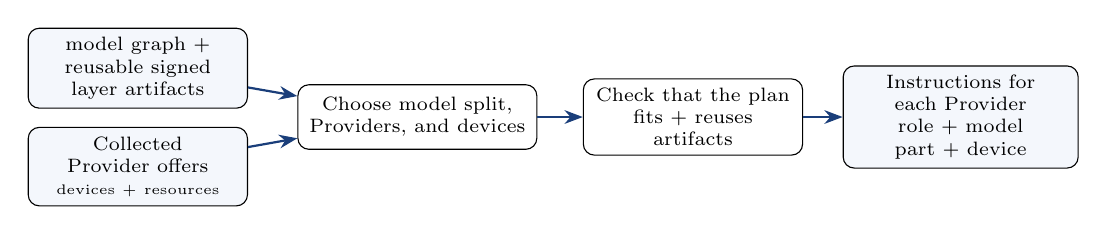
\begin{tikzpicture}[every node/.style={font=\scriptsize, align=center}]
  \node[draw, rounded corners, fill=LightBand, text width=2.55cm, minimum height=0.70cm] (graph) at (0.8,1.10) {model graph +\\reusable signed layer artifacts};
  \node[draw, rounded corners, fill=LightBand, text width=2.55cm, minimum height=0.70cm] (views) at (0.8,-0.15) {Collected\\Provider offers\\{\tiny devices + resources}};
  \node[draw, rounded corners, fill=white, text width=2.80cm, minimum height=0.82cm] (strategy) at (4.35,0.48) {Choose model split,\\Providers, and devices};
  \node[draw, rounded corners, fill=white, text width=2.55cm, minimum height=0.82cm] (validate) at (7.85,0.48) {Check that the plan\\fits + reuses artifacts};
  \node[draw, rounded corners, fill=LightBand, text width=2.75cm, minimum height=0.82cm] (plan) at (11.25,0.48) {Instructions for each Provider\\role + model part + device};
  \draw[-{Stealth}, thick, MemphisBlue] (graph) -- (strategy);
  \draw[-{Stealth}, thick, MemphisBlue] (views) -- (strategy);
  \draw[-{Stealth}, thick, MemphisBlue] (strategy) -- (validate);
  \draw[-{Stealth}, thick, MemphisBlue] (validate) -- (plan);
\end{tikzpicture}
}
\end{center}

\vspace{0.30cm}
\begin{columns}[T,onlytextwidth]
\column{0.46\linewidth}
\scriptsize
\textbf{Example decision}
\begin{itemize}
  \item stage 0 $\rightarrow$ P2 / CPU
  \item stage 1, partitions A--B $\rightarrow$ P4 / GPUs 0--1
  \item reuse signed layer artifacts already cached at P4
\end{itemize}

\column{0.51\linewidth}
\scriptsize
\textbf{Resulting execution contract}
\begin{itemize}
  \item Each Provider receives only its assigned role, model part, and device.
  \item Memory and topology are checked separately for every selected device.
  \item The same Data-flow checks apply to directly received and cached tensors.
\end{itemize}
\end{columns}

\vspace{0.12cm}
\bluebox{\scriptsize Each signed Provider offer reports available devices, capacity, and cached signed layer artifacts.}
\end{frame}

\ifshortdeck
\begin{frame}{DI Hybrid Layout and Planner Decision}
\scriptsize
\begin{columns}[T,onlytextwidth]
\column{0.54\linewidth}
\begin{center}
\textbf{Candidate $N\times\{M_i\}$ layouts}
\end{center}
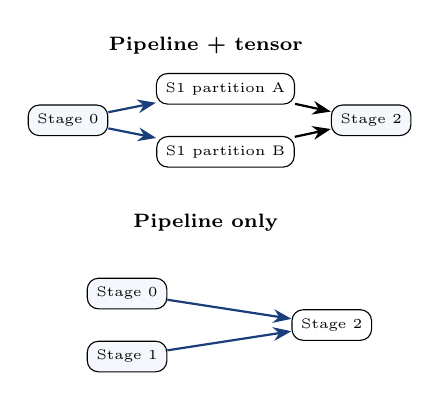
\begin{tikzpicture}[node distance=0.45cm, every node/.style={font=\tiny, align=center}]
  \node[font=\scriptsize\bfseries] at (1.75,1.90) {Pipeline + tensor};
  \node[draw, rounded corners, fill=LightBand] (b) at (0,0.95) {Stage 0};
  \node[draw, rounded corners, fill=white] (h0) at (2.0,1.35) {S1 partition A};
  \node[draw, rounded corners, fill=white] (h1) at (2.0,0.55) {S1 partition B};
  \node[draw, rounded corners, fill=LightBand] (m) at (3.85,0.95) {Stage 2};
  \draw[-{Stealth}, thick, MemphisBlue] (b) -- (h0);
  \draw[-{Stealth}, thick, MemphisBlue] (b) -- (h1);
  \draw[-{Stealth}, thick] (h0) -- (m);
  \draw[-{Stealth}, thick] (h1) -- (m);

  \node[font=\scriptsize\bfseries] at (1.75,-0.35) {Pipeline only};
  \node[draw, rounded corners, fill=LightBand] (b0) at (0.75,-1.25) {Stage 0};
  \node[draw, rounded corners, fill=LightBand] (b1) at (0.75,-2.05) {Stage 1};
  \node[draw, rounded corners, fill=white] (m2) at (3.35,-1.65) {Stage 2};
  \draw[-{Stealth}, thick, MemphisBlue] (b0) -- (m2);
  \draw[-{Stealth}, thick, MemphisBlue] (b1) -- (m2);
\end{tikzpicture}

\column{0.43\linewidth}
\textbf{Planner compares}
\begin{itemize}
  \item model/device fit,
  \item activation/collective size,
  \item RTT, bandwidth, topology,
  \item per-device capacity and reuse.
\end{itemize}
\vspace{0.18cm}
\textbf{Tradeoff}
\begin{itemize}
  \item Pipeline trades stage compute against activation transfer.
  \item Tensor sharding adds collective cost but can fit larger stages.
\end{itemize}
\end{columns}
\vspace{0.12cm}
\bluebox{\scriptsize After timely ACKs are collected, the planner assigns each model part to one Provider and device; the Provider checks capacity again before execution.}
\end{frame}
\else
\begin{frame}{Pipeline, Tensor, and Hybrid Tradeoff}
\begin{columns}[T,onlytextwidth]
\column{0.49\linewidth}
\begin{center}
\textbf{Layer-wise pipeline cut: $N=3$}

\vspace{0.25cm}
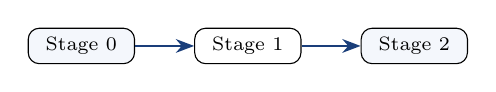
\begin{tikzpicture}[node distance=0.55cm, every node/.style={font=\scriptsize, align=center}]
  \node[draw, rounded corners, fill=LightBand, minimum width=1.35cm] (s0) {Stage 0};
  \node[draw, rounded corners, fill=white, right=0.75cm of s0, minimum width=1.35cm] (s1) {Stage 1};
  \node[draw, rounded corners, fill=LightBand, right=0.75cm of s1, minimum width=1.35cm] (s2) {Stage 2};
  \draw[-{Stealth}, thick, MemphisBlue] (s0) -- (s1);
  \draw[-{Stealth}, thick, MemphisBlue] (s1) -- (s2);
\end{tikzpicture}
\end{center}

\small
\begin{itemize}
  \item Assigns contiguous layer ranges to stages.
  \item Can span CPU and accelerator Providers.
  \item Transfers activations across stage boundaries.
\end{itemize}

\column{0.49\linewidth}
\begin{center}
\textbf{Hybrid: $N=2$, tensor partitions $\{M_i\}=\{1,2\}$}

\vspace{0.25cm}
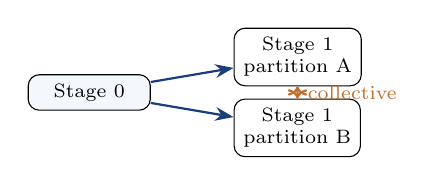
\begin{tikzpicture}[node distance=0.55cm, every node/.style={font=\scriptsize, align=center}]
  \node[draw, rounded corners, fill=LightBand, minimum width=1.55cm] (s0) {Stage 0};
  \node[draw, rounded corners, fill=white, right=1.05cm of s0, yshift=0.45cm, minimum width=1.45cm] (r0) {Stage 1\\partition A};
  \node[draw, rounded corners, fill=white, right=1.05cm of s0, yshift=-0.45cm, minimum width=1.45cm] (r1) {Stage 1\\partition B};
  \draw[-{Stealth}, thick, MemphisBlue] (s0) -- (r0);
  \draw[-{Stealth}, thick, MemphisBlue] (s0) -- (r1);
  \draw[<->, thick, AccentOrange] (r0) -- node[right]{collective} (r1);
\end{tikzpicture}
\end{center}

\small
\begin{itemize}
  \item Shards selected stages across device sets.
  \item Requires adapter-certified tensor semantics.
  \item Adds collective and redistribution cost.
\end{itemize}
\end{columns}

\vspace{0.04cm}
\bluebox{\scriptsize The planner chooses $N\times\{M_i\}$ from model constraints, reuse, per-device feasibility, topology, activation size, and network cost.}
\end{frame}

\begin{frame}{DI Planner Decision}
\vspace{-0.15cm}
\begin{center}
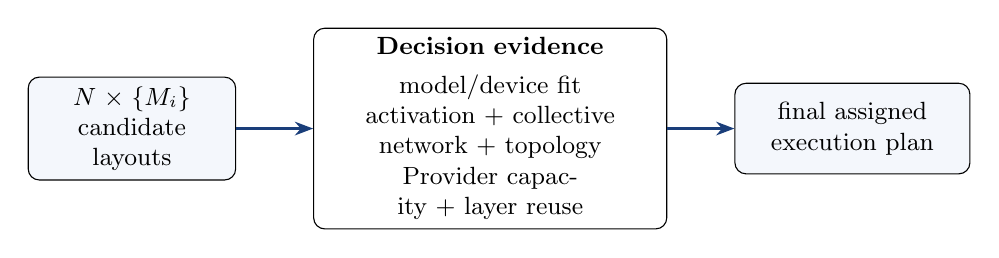
\begin{tikzpicture}[every node/.style={font=\small, align=center}]
  \node[draw, rounded corners, fill=LightBand, text width=2.4cm, minimum height=1.15cm] (candidates) at (0,0.65) {$N\times\{M_i\}$\\candidate layouts};
  \node[draw, rounded corners, fill=white, text width=4.25cm, minimum height=2.10cm] (evidence) at (4.55,0.65)
    {\textbf{Decision evidence}\\[1mm]
     model/device fit\\
     activation + collective\\
     network + topology\\
     Provider capacity + layer reuse};
  \node[draw, rounded corners, fill=LightBand, text width=2.75cm, minimum height=1.15cm] (selected) at (9.15,0.65) {final assigned\\execution plan};

  \draw[-{Stealth}, thick, MemphisBlue] (candidates) -- (evidence);
  \draw[-{Stealth}, thick, MemphisBlue] (evidence) -- (selected);
\end{tikzpicture}
\end{center}

\vspace{0.25cm}
\small
\begin{itemize}
  \item Planning begins only after all timely ACKs are collected; an ACK does not reserve hardware.
  \item Every assigned model part must fit one actual device; memory is not combined across incompatible devices.
  \item Compatible cached layers may be reused after model and topology constraints pass.
\end{itemize}
\end{frame}
\fi

\begin{frame}{Preliminary Diagnostic Experiment}
\scriptsize
Earlier role/chunk prototype on the same full-network MiniNDN harness, using a small-model ONNX \slideref{25} workload instrumented by NativeTracer; 10 successful real-ONNX runs per layout.

\vspace{0.18cm}
\begin{columns}[T,onlytextwidth]
\column{0.42\linewidth}
\textbf{Shared-backbone layout}
\vspace{0.10cm}
\begin{center}
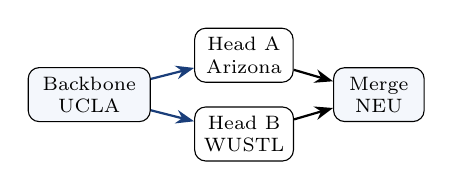
\begin{tikzpicture}[node distance=0.45cm, every node/.style={font=\scriptsize, align=center}]
  \node[draw, rounded corners, fill=LightBand, minimum width=1.55cm,
        minimum height=0.68cm] (b) {Backbone\\UCLA};
  \node[draw, rounded corners, fill=white, right=0.55cm of b, yshift=0.50cm,
        minimum width=1.25cm, minimum height=0.58cm] (h0) {Head A\\Arizona};
  \node[draw, rounded corners, fill=white, right=0.55cm of b, yshift=-0.50cm,
        minimum width=1.25cm, minimum height=0.58cm] (h1) {Head B\\WUSTL};
  \node[draw, rounded corners, fill=LightBand, right=0.50cm of h0,
        yshift=-0.50cm, minimum width=1.15cm, minimum height=0.58cm] (m) {Merge\\NEU};
  \draw[-{Stealth}, thick, MemphisBlue] (b) -- (h0);
  \draw[-{Stealth}, thick, MemphisBlue] (b) -- (h1);
  \draw[-{Stealth}, thick] (h0) -- (m);
  \draw[-{Stealth}, thick] (h1) -- (m);
\end{tikzpicture}
\end{center}
\vspace{0.10cm}
Shared backbone uses four Providers; the single-Provider control runs all four roles at UCLA.

\column{0.55\linewidth}
\textbf{Measured end-to-end latency}
\vspace{0.10cm}
\begin{center}
\tiny
\setlength{\tabcolsep}{2.8pt}
\renewcommand{\arraystretch}{1.30}
\begin{tabular}{lrrrr}
\toprule
\textbf{Layout} & \textbf{Mean} & \textbf{p50} & \textbf{p95} & \textbf{SD}\\
\midrule
Shared backbone & 259.4 & 267.7 & 283.9 & 22.1\\
Single Provider & 186.8 & 191.7 & 206.3 & 20.0\\
\bottomrule
\end{tabular}
\end{center}
\vspace{0.06cm}
\centering All values are milliseconds.
\end{columns}

\vspace{0.18cm}
\bluebox{\scriptsize For this small model, the single-Provider layout is faster because it avoids fixed intermediate-data exchange. This diagnostic does not validate the proposed V3 reuse, hybrid partitioning, multi-GPU placement, or final resource recheck.}
\end{frame}

\begin{frame}{Planned DI Validation}
\begin{itemize}
  \item \textbf{Identity and reuse:} signed layer-artifact, assembled-fragment, and loaded-runtime identities remain distinct and reproducible.
  \item \textbf{Placement/admission:} CPU and 0/1/2+ visible accelerators; per-device feasibility; no ACK-time reservation; JIT revalidation.
  \item \textbf{Execution modes:} pipeline, adapter-certified tensor, and heterogeneous $N\times\{M_i\}$ hybrid cases.
  \item \textbf{Data/security:} dependency and collective edges, direct/cache equivalence, signer/name/key-scope negative tests.
  \item \textbf{Environments:} unit/integration harness first, then MiniNDN and sealed container/Tiger qualification.
\end{itemize}
\vspace{0.25cm}
\bluebox{Evidence remains gated: the V3 design is not presented as validated until model-file reuse, local assembly, device checks, and multi-device execution gates close.}
\end{frame}

\begin{frame}{Planned Evaluation Matrix}
\scriptsize
\setlength{\tabcolsep}{3.5pt}
\renewcommand{\arraystretch}{1.12}
\begin{tabularx}{\linewidth}{
  >{\raggedright\arraybackslash}p{0.07\linewidth}
  >{\raggedright\arraybackslash}p{0.18\linewidth}
  >{\raggedright\arraybackslash}p{0.29\linewidth}
  >{\raggedright\arraybackslash}X}
\toprule
\textbf{RQ} & \shortstack[l]{\textbf{Dissertation}\\\textbf{Component}} & \shortstack[l]{\textbf{Evaluation}\\\textbf{Target}} & \shortstack[l]{\textbf{Evaluation}\\\textbf{Methodology}}\\
\midrule
RQ1 & Literature & Prior-work boundary & Literature and traceability analysis\\
\midrule
RQ2--RQ3 & Core & ACK-derived plan; role/edge admission; security, reliability, latency, overhead & Protocol tests; direct/cache tests; matched baselines\\
\midrule
RQ4 & UAV & Mobility; authorization; freshness; media; collaboration & MiniNDN/PX4 SITL \slideref{23}; selected real machines\\
\midrule
RQ5 & DI & Reuse model files; assign model parts at runtime; assemble locally; run across devices & Integration tests; MiniNDN; sealed real-model/container tests\\
\bottomrule
\end{tabularx}
\vspace{0.08cm}
\ifshortdeck
\bluebox{\scriptsize Rows state planned evidence; the earlier small-model campaign is preliminary diagnostic evidence.}
\else
\bluebox{\scriptsize Rows state planned evidence; the earlier small-model campaign is preliminary diagnostic evidence.}
\fi
\end{frame}

\ifshortdeck
\begin{frame}{Risk, Mitigation, and Timeline}
\vspace{-0.12cm}
\begin{columns}[T,onlytextwidth]
\column{0.49\linewidth}
\scriptsize
\bluebox{\centering\textbf{Primary risks and controls}}
\begin{itemize}\setlength{\itemsep}{0.02em}\setlength{\topsep}{0.05em}\setlength{\parsep}{0pt}
  \item \textbf{UAV scope:} validation workload.
  \item \textbf{Collaboration latency:} measure admission overhead.
  \item \textbf{DI data volume:} segment and measure transfers.
  \item \textbf{Variable hardware:} retain emulated baselines.
\end{itemize}

\column{0.49\linewidth}
\scriptsize
\bluebox{\centering\textbf{Spring 2027 completion path}}
\begin{description}\setlength{\itemsep}{0.02em}\setlength{\topsep}{0.05em}\setlength{\parsep}{0pt}
  \item[Aug. 2026] Plan-to-Data evaluation
  \item[Sept. 2026] UAV role/edge validation
  \item[Oct. 2026] Real-model DI/failure gates
  \item[Nov.--Dec. 2026] Evidence freeze/chair draft
  \item[Jan.--Mar. 2027] Review, defense, corrections, ProQuest
\end{description}
\end{columns}
\vspace{-0.05cm}
\begin{beamercolorbox}[rounded=true,shadow=false,sep=0.25em,wd=\linewidth]{block body}
\scriptsize Defense by mid-Feb. 2027; ProQuest: Mar. 5 target / Mar. 26 deadline; Spring 2027 graduation.
\end{beamercolorbox}
\end{frame}

\begin{frame}{Expected Contribution and Success Criteria}
\small
\begin{columns}[T,onlytextwidth]
\column{0.31\linewidth}
\begin{block}{Mechanism}
An ACK-derived collaboration plan assigns valid runtime candidates to roles and names every dependency edge.
\end{block}

\column{0.31\linewidth}
\begin{block}{Enforcement}
A Provider accepts intermediate Data only for the current request, assigned producer role, declared edge, and permitted name/key scope.
\end{block}

\column{0.31\linewidth}
\begin{block}{Evidence}
Direct/cache equivalence, same-request negative tests, matched baselines, and measured security, latency, and message overhead.
\end{block}
\end{columns}
\vspace{0.30cm}
\bluebox{\scriptsize NDNSF is the dissertation contribution; UAV and distributed inference are validation workloads that test and refine it.}
\end{frame}
\fi

\begin{frame}[plain]
\vfill
\centering
{\large\textbf{Dissertation thesis}}\\[0.25cm]
{\large NDNSF can turn ACK-derived roles and named dependencies\\into enforceable policy for direct and cached Named Data.}\\[0.35cm]
{\small The v0.1 implementation and initial evidence exist; Plan-to-Data enforcement and full validation remain proposed.}
\vfill
{\Huge Questions?}
\vfill
\end{frame}

\ifshortdeck
\else
\begin{frame}{Backup: Risk and Mitigation}
\small
\begin{tabularx}{\linewidth}{p{0.32\linewidth}X}
\toprule
\textbf{Risk} & \textbf{Mitigation}\\
\midrule
UAV prototype scope & Treat UAV as a requirements and validation workload\\
Collaboration overhead & Measure ACK/Selection/Response and Targeted paths\\
Large DI objects & Use references, segmentation, and planner cost models\\
Variable hardware & Keep MiniNDN/SITL as repeatable baselines\\
\bottomrule
\end{tabularx}
\end{frame}
\fi

\begin{frame}{Backup: UAV Validation Details}
\begin{itemize}
  \item \textbf{Targeted command lifecycle:} latency, timeout reason, explicit retry.
  \item \textbf{Typed state freshness:} telemetry, mission, video, and safety state.
  \item \textbf{Large media objects:} video and recording as signed segmented Data.
  \item \textbf{Mission recovery:} cancellation, partial recovery, and bounded role reassignment.
\end{itemize}
\vspace{0.4cm}
\bluebox{UAV validation asks whether NDNSF mechanisms support mobile, command-sensitive service use cases.}
\end{frame}

\begin{frame}{Backup: Runtime Metadata Evidence}
\small
\begin{itemize}
  \item \textbf{Adaptive admission}\\
  \textit{Configuration:} open-loop 100 RPS offered load; compare no admission control with admission-aware NDNSF.\\
  \textit{Result:} P95 latency stays at 268.12\,ms with 0.00\% timeout rate.\\
  \textit{Meaning:} providers should expose runtime capacity, not only service names.

  \item \textbf{Positive/negative ACK readiness}\\
  \textit{Configuration:} nearest provider is overloaded; the ACK-all baseline still selects it for 2209 of 2250 requests.\\
  \textit{Result:} success rises from 1.82\% to 100.00\% when negative ACKs exclude the overloaded provider.\\
  \textit{Meaning:} providers still return an ACK, but its status prevents an unavailable provider from becoming a selection candidate.
\end{itemize}
\end{frame}

\begin{frame}{Backup: User-Side Admission Control}
\small
\begin{itemize}
  \item NDNSF bounds the number of outstanding service requests before they enter the Request--ACK--Selection--Response pipeline.
  \item Each request is locally admitted, queued, or rejected according to a window updated every 500\,ms.
  \item The window grows when latency is stable, but shrinks under rising latency, timeouts, or near-full queues.
  \item Queue limits are derived from the current window, so overload protection adapts to runtime capacity instead of using one static threshold.
\end{itemize}

\vspace{0.25cm}
\begin{tabularx}{\linewidth}{>{\raggedright\arraybackslash}p{0.26\linewidth}>{\raggedright\arraybackslash}X>{\raggedright\arraybackslash}X}
\toprule
\textbf{100 RPS offered load} & \textbf{Admission enabled} & \textbf{Admission disabled}\\
\midrule
P95 latency & 268.12\,ms at 81 actual RPS & 4254.39\,ms at 100 actual RPS\\
Timeout rate & 0.00\% & 3.55\%\\
\bottomrule
\end{tabularx}
\end{frame}

\begin{frame}{Backup: NDNSF Multi-Provider Coordination}
\scriptsize
\textbf{The NDNSF paper treats provider coordination as a framework concern.}

\vspace{0.10cm}
\begin{itemize}\itemsep=0pt\parskip=0pt
  \item One Request reaches multiple authorized providers for one named service.
  \item ACK metadata reports readiness; the user selects after ACK collection.
  \item Selected providers execute and publish Responses under NDNSF security.
  \item The mechanism is framework-level coordination, not application glue.
\end{itemize}

\vspace{-0.02cm}
\begin{center}
\includegraphics[width=0.86\linewidth,height=0.39\textheight,keepaspectratio]{assets/provider_work_efficiency.png}
\end{center}
\vspace{-0.04cm}
\bluebox{\tiny Capacity-matched, block-network gated: comparable success,
5,380 duplicate provider executions avoided. This supports work efficiency,
not general mobility reliability or latency superiority.}
\end{frame}

\begin{frame}{Backup: Why Not ABE Plus Role-Certificate Authorization?}
\small
\textbf{Both designs are valid; compare their permission-management costs.}
\vspace{0.25cm}
\begin{itemize}
  \item \textbf{Alternative:} ABE protects discovery; service-role certificates and Trust Schema rules authorize execution.
  \item \textbf{NDNSF:} challenges reuse attribute-based permission management, avoiding extra service-role signing credentials.
  \item \textbf{Additional cost:} User permission DKEYs and challenge processing are not already paid for by Provider-side discovery.
  \item Both designs still validate signatures, request identity, current authority, and replay state.
\end{itemize}
\vspace{0.2cm}
\bluebox{\scriptsize Fewer credential objects do not prove lower total cost.
Compare issuance, updates, key sizes, and revocation overhead under the same permissions.}
\end{frame}

\begin{frame}{Backup: Middleware Comparison}
\textbf{gRPC \slideref{17} and ROS 2 \slideref{18} are useful, but they solve a different runtime problem.}

\vspace{0.45cm}
\begin{itemize}
  \item \textbf{gRPC:} strong RPC abstraction with name resolution, load balancing, and retry, but its channels carry messages between resolved service endpoints.
  \item \textbf{ROS 2:} strong robotics middleware built around a distributed robotics graph rather than NDN's named, cacheable Data model.
  \item \textbf{NDN advantage:} named, signed Data can be retrieved by name from providers, caches, or repositories.
  \item \textbf{NDNSF contribution:} adds authorization, ACK metadata, provider selection, replay protection, and large-data references above NDN.
\end{itemize}

\vspace{0.3cm}
\bluebox{NDNSF is not a replacement for every middleware stack; it studies what a data-centric service framework enables in dynamic, multi-provider environments.}
\end{frame}

\begin{frame}{References [1--7]}
\scriptsize
\refentry{1}{L. Zhang et al., ``Named Data Networking,'' \emph{ACM SIGCOMM Computer Communication Review}, vol. 44, no. 3, pp. 66--73, 2014.}
\refentry{2}{T. Li et al., ``A Brief Introduction to NDN Dataset Synchronization (NDN Sync),'' in \emph{Proc. IEEE MILCOM}, pp. 612--618, 2018.}
\refentry{3}{P. Moll et al., ``A Brief Introduction to State Vector Sync,'' Named Data Networking Project, Tech. Rep. NDN-0073, rev. 2, 2021.}
\refentry{4}{Z. Zhang et al., ``NAC: Automating Access Control via Named Data,'' in \emph{Proc. IEEE MILCOM}, 2018.}
\refentry{5}{C. A. Lee et al., ``Supporting Virtual Organizations Using Attribute-Based Encryption in Named Data Networking,'' in \emph{Proc. IEEE CIC}, pp. 188--196, 2018.}
\refentry{6}{C. Tschudin and M. Sifalakis, ``Named Functions and Cached Computations,'' in \emph{Proc. IEEE CCNC}, pp. 851--857, 2014.}
\refentry{7}{M. Krol and I. Psaras, ``NFaaS: Named Function as a Service,'' in \emph{Proc. ACM ICN}, pp. 134--144, 2017.}
\end{frame}

\begin{frame}{References [8--13]}
\scriptsize
\refentry{8}{M. A. ur Rehman and B.-S. Kim, ``CFEC: An Ultra-Low Latency Microservices-Based In-Network Computing Framework for Information-Centric IoVs,'' \emph{IEEE Transactions on Services Computing}, vol. 17, no. 6, pp. 3199--3212, 2024.}
\refentry{9}{M. Krol et al., ``RICE: Remote Method Invocation in ICN,'' in \emph{Proc. ACM ICN}, pp. 1--11, 2018.}
\refentry{10}{D. Meirovitch and L. Zhang, ``NSC---Named Service Calls, or a Remote Procedure Call for NDN,'' Named Data Networking Project, Tech. Rep. NDN-0074, rev. 1, 2021.}
\refentry{11}{M. Imran et al., ``MIA-NDN: Microservice-Centric Interest Aggregation in Named Data Networking,'' \emph{Sensors}, vol. 23, no. 3, Art. no. 1411, 2023.}
\refentry{12}{K. Nichols, ``Lessons Learned Building a Secure Network Measurement Framework Using Basic NDN,'' in \emph{Proc. ACM ICN}, pp. 112--122, 2019.}
\refentry{13}{R. Tourani et al., ``Towards Security-as-a-Service in Multi-Access Edge,'' in \emph{Proc. ACM/IEEE SEC}, pp. 358--363, 2019.}
\end{frame}

\begin{frame}{References [14--21]}
\scriptsize
\refentry{14}{M. Król et al., ``Compute First Networking: Distributed Computing Meets ICN,'' \emph{ACM ICN}, 2019.}
\refentry{15}{C. Barrios et al., ``CaSCON: Cache-Assisted Service Composition Orchestration Leveraging NDN,'' \emph{IEEE SMARTCOMP}, 2025.}
\refentry{16}{Y. Yu et al., ``Schematizing Trust in Named Data Networking,'' \emph{ACM ICN}, 2015.}
\refentry{17}{gRPC Authors, ``Core Concepts, Architecture and Lifecycle,'' gRPC Documentation, accessed July 2026.}
\refentry{18}{S. Macenski et al., ``Robot Operating System 2: Design, Architecture, and Uses in the Wild,'' \emph{Science Robotics}, 2022.}
\refentry{19}{S. Dulal et al., ``Enhancing NAC-ABE to Support Access Control for mHealth Applications and Beyond,'' \emph{arXiv:2311.07299}, 2023.}
\refentry{20}{C. Marxer et al., ``Access-Controlled In-Network Processing of Named Data,'' \emph{ACM ICN}, 2016.}
\refentry{21}{S. D. Fu et al., ``Toward Data-Centric Service Composition,'' \emph{ACM HotNets}, 2024.}
\end{frame}

\begin{frame}{References [22--25]}
\scriptsize
\refentry{22}{Mini-NDN Developers, ``Mini-NDN: A Mininet-Based NDN Emulator,'' project documentation, accessed August 2026.}
\refentry{23}{PX4 Development Team, ``Simulation: Software in the Loop (SITL),'' \emph{PX4 User Guide}, accessed August 2026.}
\refentry{24}{Named Data Networking Project, ``Repo Protocol Specification,'' repo-ng documentation, accessed August 2026.}
\refentry{25}{ONNX Project, ``Open Neural Network Exchange Intermediate Representation Specification,'' ONNX documentation, accessed August 2026.}
\end{frame}

\end{document}
